\documentclass{ucsdreport}
\usepackage{hyperref}
\graphicspath{{./images/}}
%************************************************************
% ABOUT THIS HOMEWORK
\def\course{CSE Honors Thesis}      %Course
\def\thetitle{Citizen-Centric Infrastructure with an 
            Artificial Intelligence and Data Science
            Backbone}               % Report Title
\def\Headauthor{Yuling Shi}         % Header Authors of work
\def\date{\today}                         % Date

% DOCUMENT START
\begin{document}

% TITLE PAGE
\begin{center}
    \vspace*{1.5cm}
    % University Logo
    
\includegraphics[scale = 0.10]{UCSDseal.png}\\[1.75cm]
    % University Name
    \textsc{\color[RGB]{0, 51, 102}\LARGE{University of California San Diego}}\\[1cm]
    \textsc{\Large{\course}}\\[.5cm]
    \textsc{\Large{\thetitle}}\\[.5cm]
    \textsc{\date}\\[2cm]
    \Large{
    \begin{tabular}{L{4cm} R{4cm}}
        \textit{Author} &  \textit{Email}\\
        \hline
        % author names and PID
        Yuling Shi & yus252@ucsd.edu \\
    \end{tabular}
    }
\end{center}
\thispagestyle{empty}
\pagebreak

% TABLE OF CONTENTS
\tableofcontents{}
\pagebreak

% REPORT START
%%%%%%%%%%%%%%%%%%%%%%%%%%%%%%%%%%%%%%%%%%%%%%%%%%%%%%%%%%%%%%%%%%%%%%%%%%%%%%%
%%%%%%%%%%%%%%%%%%%%%%%%%%%%%%%%%%%%%%%%%%%%%%%%%%%%%%%%%%%%%%%%%%%%%%%%%%%%%%%
%%%%%%%%%%%%%%%%%%%%%%%%%%%%%%%%%%%%%%%%%%%%%%%%%%%%%%%%%%%%%%%%%%%%%%%%%%%%%%%


\begin{spacing}{2}
\section{Acknowledgement}

\tab First, I would like to thank my research supervisor, Professor Henrik I. 
Christensen, for his encouragement and support on my honors projects, COVID
Maps and OASIS, and my Computer Science studies at the University of California
San Diego. In the past two years, he assisted in every step throughout the
process, helping me with both my academic and professional goals. 

\tab  I also want to thank my teammates, including Professor Eliah Aronoff-Spencer, 
Professor Nadir Weibel, Stella Li, Paul Zhu, Alex Wenzel, Yingxi Lin, 
Nicolás di Tada, and his team at InSTEDD. They contributed to OASIS in various
ways, including designing and programming.

\tab  Finally, I would like to thank my friends and family for their data contribution 
in the early stage of the two projects and their psychological support, 
especially during the quarantine. 

\tab  Without any of those people, I could not have accomplished my thesis. I will always 
remember the hard time during the COVID-19 pandemic and appreciate the love 
and support I received.

\end{spacing}
\newpage
%%%%%%%%%%%%%%%%%%%%%%%%%%%%%%%%%%%%%%%%%%%%%%%%%%%%%%%%%%%%%%%%%%%%%%%%%%%%%%%
%%%%%%%%%%%%%%%%%%%%%%%%%%%%%%%%%%%%%%%%%%%%%%%%%%%%%%%%%%%%%%%%%%%%%%%%%%%%%%%
%%%%%%%%%%%%%%%%%%%%%%%%%%%%%%%%%%%%%%%%%%%%%%%%%%%%%%%%%%%%%%%%%%%%%%%%%%%%%%%
\begin{spacing}{2}
\section{Abstract} 
\tab Citizen-centricity is a bottom-up approach that empowers citizens to engage
in and address different natural and societal challenges. Sometimes people may 
refer it as citizen science. As COVID-19 is
raging the world, we tried to build a citizen-centric infrastructure that
allows every citizen to fight against COVID-19, exploring how citizens can
contribute to, what user information is necessary, and what technology tools
are needed. We started with contacting tracing by building a website, COVID
Maps, to let users share their GPS history data and inform users of the
population's intersectionality and density. Later, we created OASIS, a website
for users to share their data, find trustworthy resources to deal with 
COVID-19, and get insights generated from COVID-19 stories shared by users.
In the thesis, I will talk about the problems our team have met in those projects 
and how to address them using different tools. I will also talk about lessons
learned from the study and outlooks for future research. 
\end{spacing}
\newpage

%%%%%%%%%%%%%%%%%%%%%%%%%%%%%%%%%%%%%%%%%%%%%%%%%%%%%%%%%%%%%%%%%%%%%%%%%%%%%%%
%%%%%%%%%%%%%%%%%%%%%%%%%%%%%%%%%%%%%%%%%%%%%%%%%%%%%%%%%%%%%%%%%%%%%%%%%%%%%%%
%%%%%%%%%%%%%%%%%%%%%%%%%%%%%%%%%%%%%%%%%%%%%%%%%%%%%%%%%%%%%%%%%%%%%%%%%%%%%%%
\section{Introduction}

%%%%%%%%%%%%%%%%%%%%%%%%%%%%%%%%%%%%%%%%%%%%%%%%%%%%%%%%%%%%%%%%%%%%%%%%%%%%%%%
\subsection{Citizen-Centricity}
At present, there are many natural and societal challenges on the planet, from 
the COVID-19 pandemic to disparity of wealth. There is an urgent need for 
actions to address those issues. However, how do we solve those problems?

The top-down approach applied by governments engages in system-level changes 
driven by policy and operational directives (Gallup, 2018). It could bring 
widespread changes to address natural and societal issues. However, it demands
complicated governmental procedures and a long time for implementation, passing
from the decision-maker down to the general population. Even though policy 
changes are successfully passed, whether citizens follow the rule or not is 
another story. 

On the contrary, the bottom-up approach, which may have a limited impact that 
each person brings (Gallup, 2018). However, solving the world’s problems is a 
big task that cannot be accomplished by a single person. Therefore, we should pursue such 
efforts using a citizen-centric approach, where people are empowered to engage 
and address these challenges. Through more recycling carried out by individuals
in California, we lessen the impact of our throw-way culture on the environment, 
creating a cleaner, healthier, and more sustainable environment (Klug, 2020). 
In African countries, public participation in regulating mining ensures that 
the overall management of exploiting mineral resources is sustainable 
(R. Gisore, Z. Matina, and N. KenyA, 2015). At present, journalism transformed 
from newsroom cultures to a new communicative orientation, relying mostly on
social networks to immediately reach tons of audiences who can react to a 
particular policy, issue, and topic (Kramp L., Loosen W., 2018). These are
great examples of how individuals are empowered to have a significant impact 
on their daily lives. This is where we started. As COVID-19 is raging
the world, we are interested in tools through which citizens can share 
information with the broad community to solve these challenges, information 
necessary for the solution, and tools to enable such processes. 


%%%%%%%%%%%%%%%%%%%%%%%%%%%%%%%%%%%%%%%%%%%%%%%%%%%%%%%%%%%%%%%%%%%%%%%%%%%%%%%
\subsection{Data from Citizens}
There are multiple ways that citizens can contribute to a solution. For 
example, citizens can donate to an NGO for healthcare, volunteer for tree 
planting, clean the trash for local communities, or join protests for social
justice, such as the Civil Right Movement in the 1950s, the Orange Revolution 
in 2004, and Black Lives Matter started in 2013. Of course, when everyone 
carries out practical actions in real life, there is a considerable improvement
in the environment and society. However, from a computer science perspective, 
we seek a more scientific, systematic, and cost-effective way to address those
challenges. Most importantly, each individual is a data source. From citizens' 
experiences, such as what issues they met, how they dealt with it, and what 
the result of their solution was, we can generate insights around those issues. 

For example, some citizen-centric initiatives, which encourage the general 
population to take action, apply different strategies to address water 
pollution worldwide. By investigating what they are doing, how they motivate 
citizens to contribute to the solution, how many citizens get involved, what 
the result of citizens' engagement is, and so on, data scientists can determine
what makes a citizen-centric environmental organization succeed in addressing
water pollution. 

A most recent example could be evaluating the impact of COVID-19 on people's 
daily life through social networking services and generating insights to fight
against COVID-19. Tons of data points could be extracted from social media 
like Twitter, where users share their experiences and feelings about COVID-19.
The DARPA Network Challenges illustrated the critical roles that the internet 
and social networking play in the real-time communications, wide-area 
collaborations, and particle actions required to solve board scope,
time-critical problems (DARPA, 2009).
Applying natural language processing techniques, such as finding the most 
popular topics, the trend of hot topics, co-occurrence and networks of words, 
and sentiment analysis on users' posts, scientists would know what people need. 

In conclusion, citizens are an abundant and diverse database that scientists
could always explore.Therefore, we decided to apply citizen science, in which 
public participants engage in any part of the scientific process -- promote
public engagement as a mechanism to address complex problems (ASH CENTER, 2017). 
Specifically, we want to develop a citizen-centric infrastructure for data
collection to deal with natural and societal challenges by  artificial 
intelligence algorithms and data science methods. 

%%%%%%%%%%%%%%%%%%%%%%%%%%%%%%%%%%%%%%%%%%%%%%%%%%%%%%%%%%%%%%%%%%%%%%%%%%%%%%%
\subsection{Problem Statement}
Many natural and societal challenges are going on globally, from wildfires in 
California, social justice in the U.S. to COVID-19 pandemic, and global 
warming. Based on the emergency and scale, we started with COVD-19 pandemic. 

The COVID-19 pandemic presents a global threat never experienced in modern 
times. At the moment, the therapeutic strategies to deal with the infection are
only supportive, and prevention aimed at reducing transmission in the community
is our best weapon. Thus, further studies are needed to understand the 
mechanisms of transmission.

Simultaneously, as COVID-19 has affected every aspect of people’s lives, 
including economics, healthcare, and politics, how to help people get back to 
normal life becomes another problem. However, how severe is each aspect on 
which people have been affected by COVID is not clear. Therefore, to help 
people return to normal life requires more feedback from the public. 

Finally, we should consider applying what we have learned from COVID-19 to 
solve other natural challenges, like global warming. Both COVID-19 and climate 
change could be catastrophic for humanity. While COVID-19 disrupts societies in
just a few weeks, climate change is much slower acting but ultimately more 
severe. (Cho, 2020) As we confront the current crisis, 
can we learn from it to deal with climate change? What can we learn about 
citizen-centric activities to address a challenge? 

Therefore, this project investigates the situation, insights, and the impact 
of COVID-19 to fight against it and applies what we learn here to deal with 
other natural challenges, such as global warming. There are two main website 
products involved: COVID-19 Maps and OASIS. COVID-19 Maps was created around 
April 2020, where users can share their GPS data from Google Map Timeline and 
get informed of the risks of getting COVID-19 in different regions. It aims 
to analyze the level of social distancing through the intersectionality and 
density of populations. However, as COVID-19 Maps relates privacy concerns, 
we have to resort to another way to control the virus. Consequently, we started
OASIS, which allows users to view up to date COVID-19 data, get personalized 
COVID-19 resources, share their personal stories about COVID-19, and view 
others’ stories all over the world on one single map. The methodology for 
generating insights of COVID-19 is analyzing self-reported personal stories 
about COVID-19 and personal information on OASIS by Natural Language 
Processing(NLP) and data science methods. Besides, through OASIS development, 
we will learn how to build a citizen-centric infrastructure with an artificial
intelligence and data science backbone to implement a similar infrastructure 
for future natural challenges. 


%%%%%%%%%%%%%%%%%%%%%%%%%%%%%%%%%%%%%%%%%%%%%%%%%%%%%%%%%%%%%%%%%%%%%%%%%%%%%%%
\subsection{Report Outline}
Firstly, we will illustrate how we build up the website, COVID Maps, and a
related framework, GIS System, including data capturing, data processing, 
data storage, and data displaying. We will also discuss its limitations, 
mainly on privacy concerns, and how we tried to avoid the same issues in the
next project, OASIS. 

About OASIS, we will focus on the principles to create a simple but engaging 
online platform for citizens to share data and get reliable information about 
COVID-19 and what possible ways that we can achieve those principles. Next, we
will go through tools that helped us achieve those principles, address privacy
concerns, and manage the development team. 

At last, what work has been done in the two projects will be summarized. We will 
look at what we have learned from the projects and future research questions 
for citizen-centric science. 

\newpage



%%%%%%%%%%%%%%%%%%%%%%%%%%%%%%%%%%%%%%%%%%%%%%%%%%%%%%%%%%%%%%%%%%%%%%%%%%%%%%%
%%%%%%%%%%%%%%%%%%%%%%%%%%%%%%%%%%%%%%%%%%%%%%%%%%%%%%%%%%%%%%%%%%%%%%%%%%%%%%%
%%%%%%%%%%%%%%%%%%%%%%%%%%%%%%%%%%%%%%%%%%%%%%%%%%%%%%%%%%%%%%%%%%%%%%%%%%%%%%%
\section{Contact Tracing}
Social distancing can effectively decrease the disease transmission (Cascella, 
Rajnik, Cuomo, et al., 2020). Therefore, contact tracing is one of the most 
effective way to help people to avoid getting COVID-19. It is a process to 
identify, monitor, and support individuals who may have been exposed to a
person with a communicable disease, such as COVID-19 (CDC, 2020). We 
decided to start from there.

%%%%%%%%%%%%%%%%%%%%%%%%%%%%%%%%%%%%%%%%%%%%%%%%%%%%%%%%%%%%%%%%%%%%%%%%%%%%%%%
\subsection{GIS System}
A geographic information system(GIS) is a conceptualized framework that can 
capture and analyze spatial and geographic data (Huisman and By, 2009).
To develop the 
website COVID-19 Maps to display the population's intersectionality and density,
we used the GIS system to capture, process, store, and display data. Tools 
involved are website development in Javascript, Google Maps Timeline, Firebase,
and Mapbox. 

%%%%%%%%%%%%%%%%%%%%%%%%%%%%%%%%%%%%%%%%%%%%%%%%%%%%%%%%%%%%%%%%%%%%%%%%%%%%%%%
\subsection{Data Capturing}
COVID-19 means contacting tracing on a constant and large scale. Hence, 
smartphones, which people can easily bring everywhere, would become the 
container of a contracting tracking app. Developing a mobile app by ourselves 
to track people's whereabouts seems a great way to implement contact tracking. 
However, it is not accurate enough to identify with whom people may have gotten
in touch. 

Other kinds of contacting tracking apps use Bluetooth to communicate with other
Bluetooth-enabled devices nearby, generating an anonymous alert to other users 
based on proximity and length of exposure ( C. N. Service. 2020). The 
University of California Health is piloting this smartphone technology that 
notifies users if they have had a high-risk COVID-19 exposure. However, users 
cannot prevent from getting COVID-19 with this solution. 

Therefore, we decided to get the existing GPS data from Google and Apple that 
provide more precise GPS tracking and keep tracking users' locations if we got
permission from users. Since Apple does not provide an API for getting users' 
location, it is not easy to get those data. Simultaneously, Google does not 
offer such an API either. However, Google supports users to download their 
location history through Google Takeout. One problem with it is that the 
downloaded file contains all the user locations, which is a significant burden
when processing data. Besides, only location history for the past 14 days is 
needed because the approximate number of days for the symptoms to appear after 
a person got infected is 14 days. Another problem with Google Takeout is that 
users need to book their location history files, and exporting data takes hours 
long. Thus, how to get data by day and simplify the process becomes the most 
challenging part. 

According to the tutorial Map Location History by Geffert in 2017, exporting 
GPS data on a particular page from Google Maps could be done by a python script. 
The tutorial shows how to get a user's cookie when logged into the Google Maps
website and request an encoded URL with the cookie to download the user's GPS
data as KML files. (KML, an XML notation for expressing geographic annotation and 
visualization within two-dimensional maps and three-dimensional Earth browsers) 
The method helps to get data by day but is still too complicated.

Based on the cookie-related mechanism, we improved on the process. When a user 
logs into the Google Account, Google OAuth 2.0 generates a security cookie that 
contains the user's login information. With this cookie, users can direct to 
other Google services without logging in. Also, a hyperlink embedded in the 
website could automatically direct to a URL when being clicked. Therefore, we 
created the website, COVID Maps, directing users to log into the website with 
their Google accounts and click on a hyperlink under which 14 encoded URLs for
14 days' KML files are hidden. By opening a blank window and changing the URLs 
for that window, 14 URLs will be opened one by one in the background, 
downloading those KML files. 

%%%%%%%%%%%%%%%%%%%%%%%%%%%%%%%%%%%%%%%%%%%%%%%%%%%%%%%%%%%%%%%%%%%%%%%%%%%%%%%
\subsection{Data Processing}

After downloading KML files from Google Maps Timeline, users can upload their 
files to COVID-19 Maps. KML is a file format used to display geographic data 
in an Earth browser such as Google Earth. However, it is not compatible with 
more complex and flexible geodata displaying, like heatmap, circles, and layers.
Mover, those KML files contain users’ personal information, such as email, 
home address, and name. Thus, instead of storing those KML files, COVID-19 Maps
only extracts the necessary features: coordinates and timespan. Both of them are 
under the tag \texttt{<Placemarker>}. To simplify the documentation, we have:

\begin{verbatim}
<Placemarker>
    <name> ... </name>
    </address>
    <ExtendedData> ... </ExtendedData>
    <description> ...</description> 
    <LineString>
        <altitudeMode>
        <extrude>
        <tessellate>
        <coordinates> lng, lat, height, lng, lat, height, ...</coordinates>
    <LineString>
    <TimeSpan>
        <begin> dateTime </begin>
        <end> dateTime </end>
    </TimeSpan>
</Placemarker> 
\end{verbatim}

Or 

\begin{verbatim}
<Placemarker>
    <name> ... </name>
    <address> ... </address> 
    <ExtendedData> ... </ExtendedData>
    <description> ... </description> 
    <Point>
        <altitudeMode>
        <extrude>
        <tessellate>
        <coordinates> lng, lat, height, lng, lat, height, ... </coordinates>
    <Point>
    <TimeSpan>
        <begin> dateTime </begin>
        <end> dateTime </end>
    </TimeSpan>
</Placemarker> 
\end{verbatim}

Whether it is \texttt{<Point>} or \texttt{<LineString>} depends on if the 
geodata is a static point or a line of movement. Based on XML documentation,
KML files can be easily parsed into GEOJSON objects.

%%%%%%%%%%%%%%%%%%%%%%%%%%%%%%%%%%%%%%%%%%%%%%%%%%%%%%%%%%%%%%%%%%%%%%%%%%%%%%%
\subsection{Data Storage}
Based on the simple query capacities, fast implementation, and demand for JSON 
objects, we applied Firebase to store that data. In the beginning, we have two
main references: /Points and /Users. /Users contain different usernames (key), 
each of which has multiple data points. /Points contain different data 
points(key), each of which has one corresponding user. The database schema 
is as follows:
\begin{verbatim}

{
    "Database": {
        "Points": {
            "point1_key": {
                "begin": "date_time",
                "end": "data_time",
                "lat": "lat_val",
                "lng": "lng_val",
                "user": "user1_key"
            },
            "point2_key": {
                "begin": "date_time",
                "end": "data_time",
                "lat": "lat_val",
                "lng": "lng_val",
                "user": "user1_key"
            },
            "point3_key": ...
        },
        "Users": {
            "user1_key": {
                "point1_key": "",
                "point2_key": ""
            },
            "user2_key": {
                "point3_key": ""
            }
        }
    }
}

\end{verbatim}

\begin{figure}[H]
    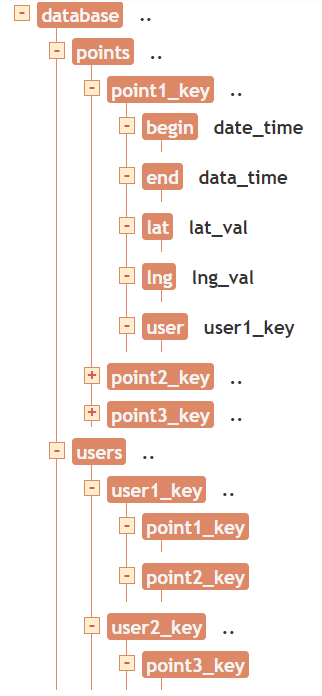
\includegraphics[scale=0.45]{images/database1.png}
    \caption{Database Schema}
\end{figure}

The solution is clean and straightforward. When showing the population's 
density, we just put all the points from /Points onto the heatmap. However, 
the time for map render becomes longer and longer when showing the 
intersectionality of people's trajectories. To show the intersectionality of 
users' trajectories, we calculate the distance between every two geographical 
points by the Haversine formula and mark their midpoint as intersection if the 
distance is smaller than 50 meters and the two points were generated in the 
same hour. Thus, the runtime is $C(2, n) = O(n^2)$. As the number of data points
and users increases, the rendering time will grow exponentially. Consequently, 
we need to improve the runtime. 

First, we changed the database. The new database schema is as follows:

\begin{verbatim}

{
    "Database": {
        "Points": {
            "country": {
                "state": {
                    "city": {
                        "zipcode": {
                            "date1": {
                                "point1_key": {
                                    "begin": "date_time",
                                    "end": "date_time",
                                    "lat": "lat_val",
                                    "lng": "lng_val",
                                    "user": "user_key"
                                },
                                "point2_key":...
                            },
                            "date2": ...(same as previous date1)
                        }
                    }
                }
            }
        },
        "Users": {
            "user1_key": {
            "Dates": {
                "date1": "",
                "date2": ""
            },
            "Points": ...(same structure as previous Points)
        },
            "user2_key": ...(same structure as previous user1_key) 
            "user3_key": ...(same structure as previous user1_key) 
        }
        "Covid": {
            "user1_key": ...(same structure as previous user1_key)
            "user2_key": ...
        }
    }
}

\end{verbatim}

The arrows of the same color have the same structure. After parsing the XML 
files, COVID-19 Maps conducts reverse geocoding on the coordinates to get the 
country, state, city, and zip code. References Dates for Users and Covid at the
root reference is added. Dates records the dates of the location history that 
the user uploaded. Based on Dates, COVID-19 Maps can remind users to share 
their location history if they did not share their location history in the past
14 days. Covid keeps track of the users who have already gotten COVID-19, as a 
result of which users who have contacted the infected users will get anonymous 
notification from the website.

\begin{figure}[H]
    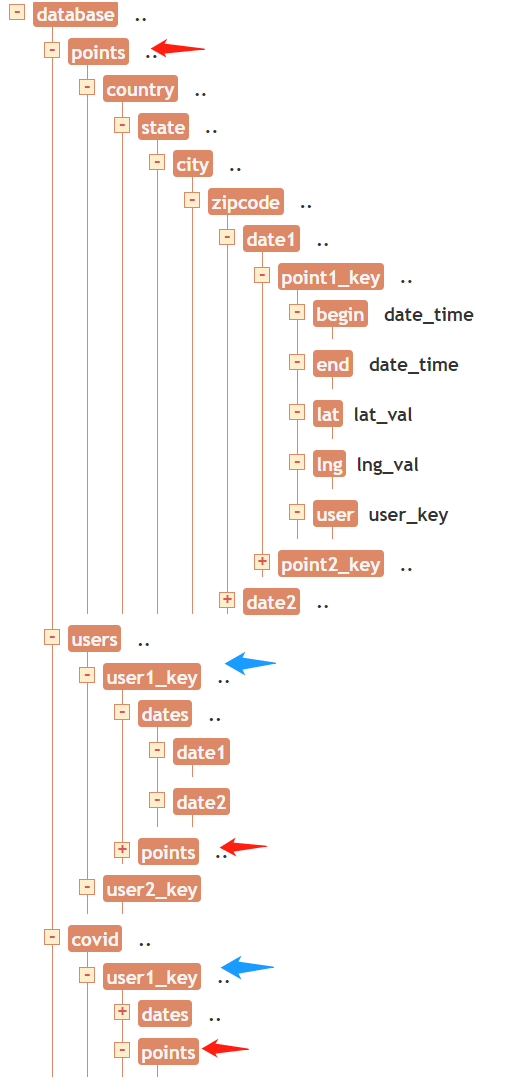
\includegraphics[scale=0.5]{images/database2.png}
    \caption{Database Schema}
\end{figure}

Besides the changes in the database, we redesigned the algorithm to find out 
intersections of people's trajectories. Querying on the database from the top 
to the bottom layer returns arrays of points at each zip code. Next, sort each
array based on latitude and then loop through the array, checking if one point
is within 50 meters to the next point and two points happen in the same hour. 
Finally, sorting each array based on longitude and doing the same check to find
the intersections. Hence, the runtime for rendering the map of intersection 
nations is $O(nlogn/C)$, where C is the number of zip codes. Even though it is 
possible to calculate the intersection between two close points as two 
intersections and miss some points on a zip-code region's margin, overall, the 
algorithm's efficiency and accuracy are well-balanced. 

%%%%%%%%%%%%%%%%%%%%%%%%%%%%%%%%%%%%%%%%%%%%%%%%%%%%%%%%%%%%%%%%%%%%%%%%%%%%%%%
\subsection{Data Displaying }
There are three popular Map APIs: Mapbox API, OpenStreetMap API, and
Google Maps API. Google Map API is heavy to render, not visually represented to 
display data, and expensive for beginners. The OpenStreetMap API is free. 
However, it is meant for map-editing purposes and has incomplete documentation.
The most commonly used standard format designed for representing simple 
geographical features is GEOJSON. Therefore, we chose Mapbox for data 
visualization. 

%%%%%%%%%%%%%%%%%%%%%%%%%%%%%%%%%%%%%%%%%%%%%%%%%%%%%%%%%%%%%%%%%%%%%%%%%%%%%%%
\subsection{Result}
COVID Maps offers 3 kinds of maps:
\begin{enumerate}
    \item Density Map: shows the activity level of a community by drawing out 
    all the trajectories of all users in the past 14 days.
    \item Intersection Map: shows how good social distancing is in a community
    based on the number of people visiting the same place at the same time.
    \item shows the contact between a user and all the COVID19 cases reported to
    this website.
\end{enumerate}
\begin{figure}[H]
    \centering
    \fbox{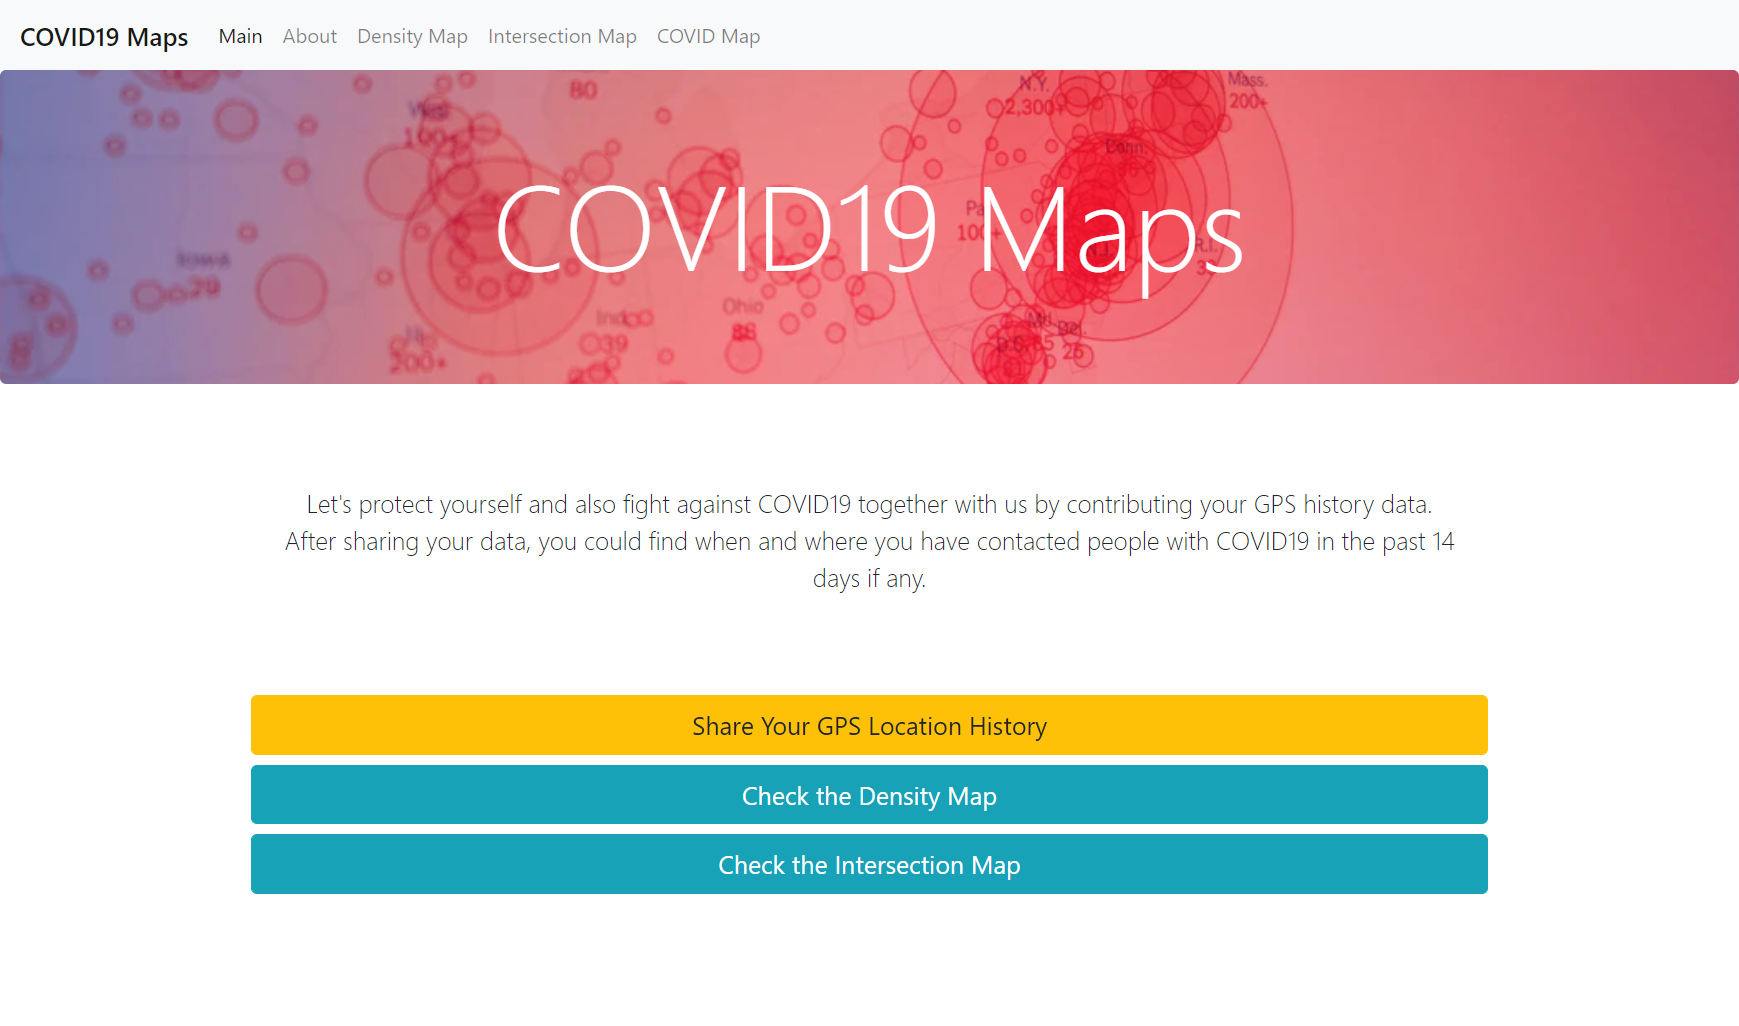
\includegraphics[scale=0.4]{images/main_page.png}}
    \caption{The Main Page}
\end{figure}

The Intersection Map shows the intersections of users' traveling trajectories 
in the past 14 days as a heatmap. However, since there are only 13 users in the 
database, no intersection exists in their traveling trajectories. Therefore, the 
Density Map is empty. 

The Density Map displays all users' raveling trajectories in the past 14 days 
as a heatmap. An example of the Density Map 05/03/2020 to 05/17/2020 shows as 
follows:

\begin{figure}[H]
    \centering
    \fbox{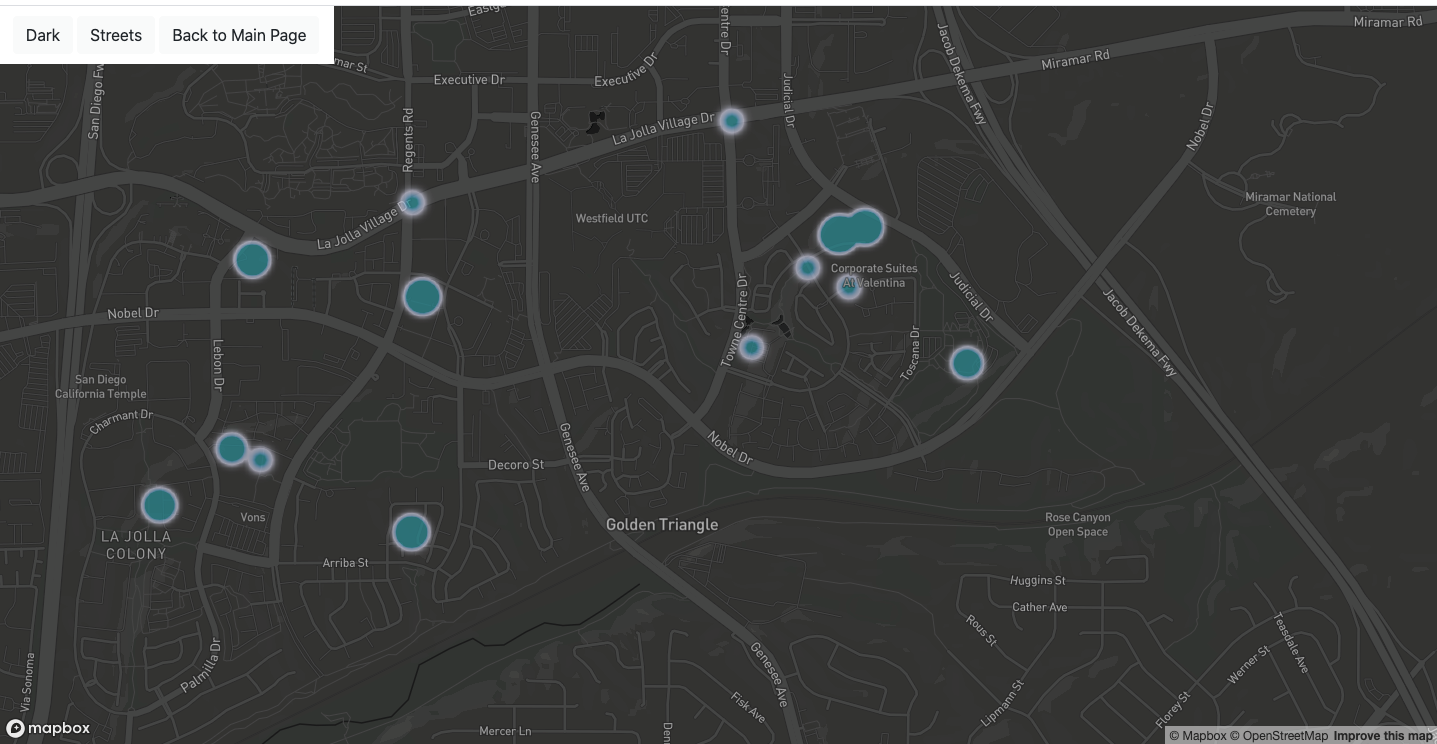
\includegraphics[scale=0.4]{images/density_map.png}}
    \caption{The Density Map}
\end{figure}

The Personal COVID19 Map marks a user's GPS points in the past 14 days as green 
circles but marks where that user met people self-reported with COVID-19 on the
same day as a red circle. Since none of the 13 users are self-reported with 
COVID-19, circles shown on every user's Personal Map are green. 

\begin{figure}[H]
    \centering
    \fbox{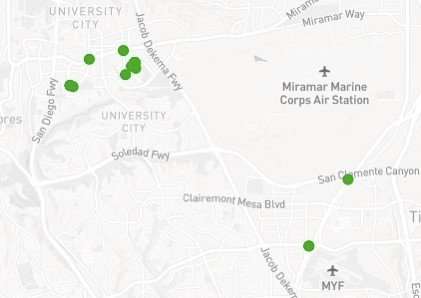
\includegraphics[scale=0.9]{images/personal_map.jpg}}
    \caption{The Personal COVID Map}
\end{figure}


%%%%%%%%%%%%%%%%%%%%%%%%%%%%%%%%%%%%%%%%%%%%%%%%%%%%%%%%%%%%%%%%%%%%%%%%%%%%%%%
\subsection{Limitations}
The contact tracing strategy to prevent the spread of COVID-19 seems useful. 
However, there are three main obstacles of the project.

Firstly, the user interface and user experience designs are not simple enough 
for the users to share. COVID-19 Maps is developed by only one software 
developer(Yuling Shi, the author). Even though it has the basic functionality, 
it is not visually 
satisfying, inefficiently directing users to get their location histories 
from Google Map Timeline. It is not user friendly. The process for data sharing
needs users to download their location history from Google Map Timeline and 
then upload it to COVID-19 Maps. 

\begin{figure}[H]
    \centering
    \fbox{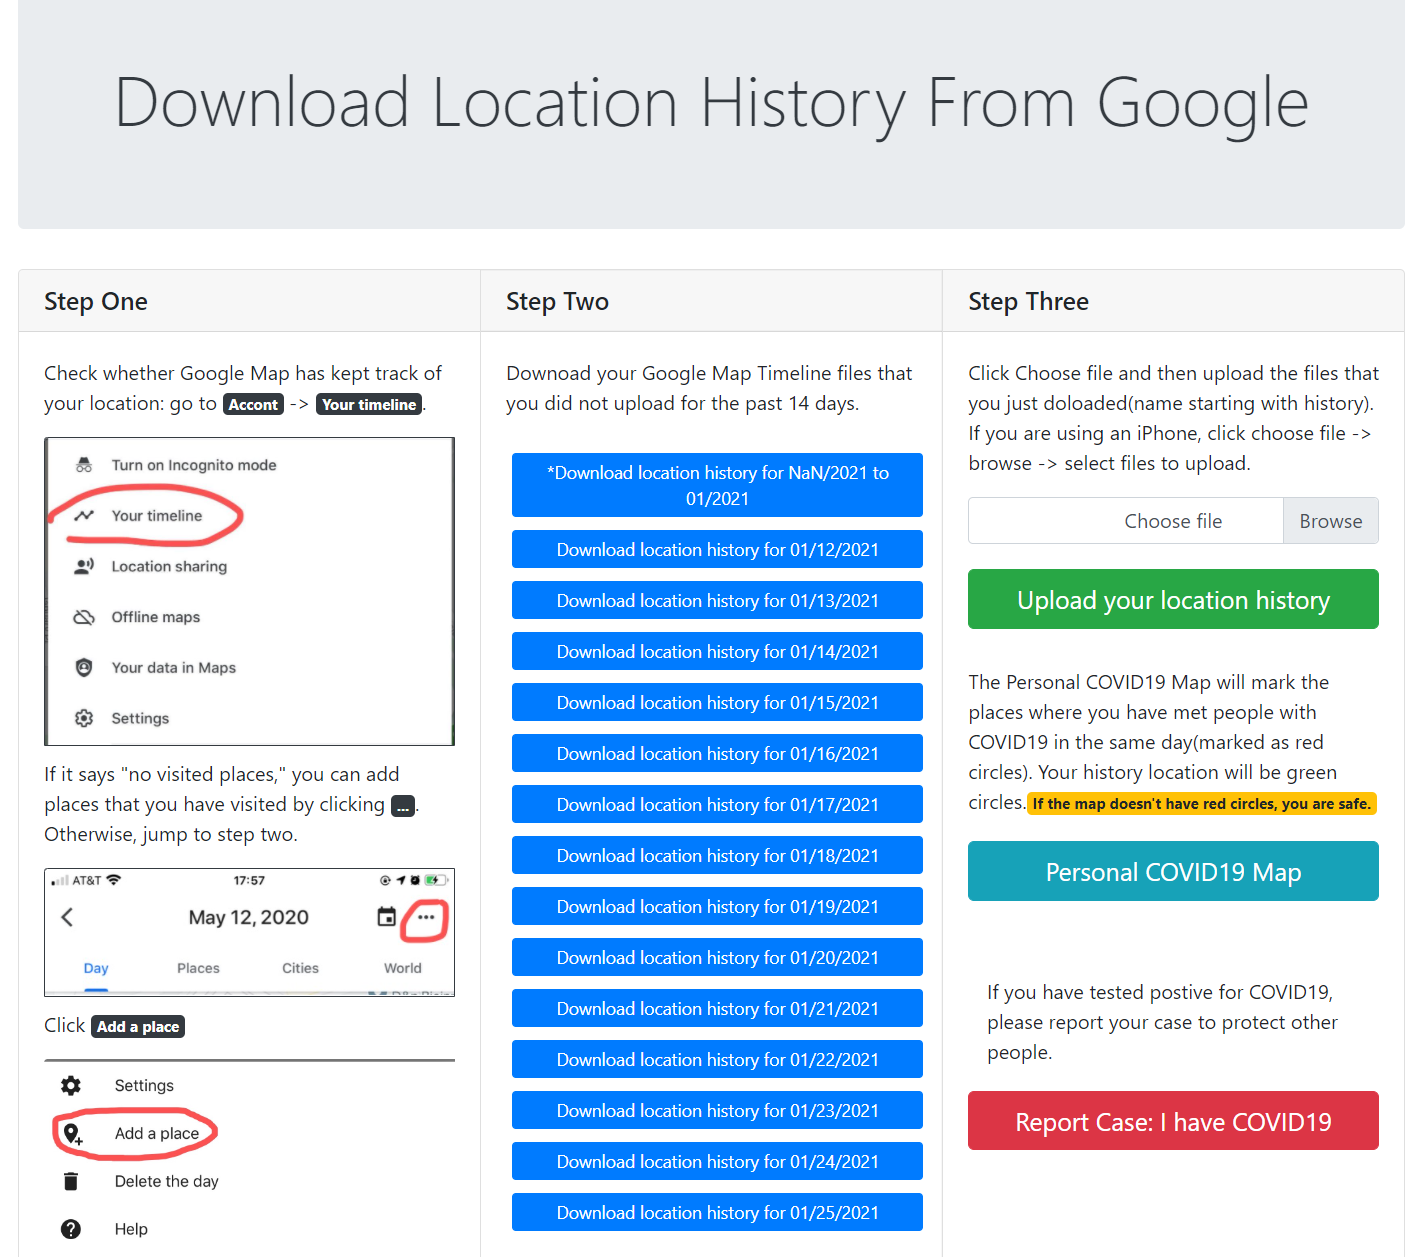
\includegraphics[scale=0.5]{images/share_page.PNG}}
    \caption{The User Interface for Data Sharing}
\end{figure}

Secondly, Google Maps does not provide an API for user location history. We 
cannot directly access users' location history but provide a way for users to 
download their location histories through authentication cookies. It makes a 
universal contact tracing app hard to be implemented. As a result, different 
governments, organizations, institutions, and companies invent their contact 
tracing app, attracting users to different platforms and having limited 
amounts of users on each product. 

Thirdly, privacy concern is the most significant issue. No matter how 
cryptography and security of the system is, citizens always have concerns
about their privacy. Feedback provided by around 20 beta testing users shows 
that the most important reason why users are not interested in COVID-19 Maps is
that they do not want to share their private information, especially locations. 
Even though Google provides such an API for the third party to access the user's
location history, if users do not open the Google Maps Timeline feature, their
location history is still blank. 

Based on the three limitations of COVID-19 Maps, we had to resort to another 
way to build a citizen-centric infrastructure that makes people more likely to 
share their experiences and information and utilize those data to generate 
insights for COVID by AI and data science methods. 

%%%%%%%%%%%%%%%%%%%%%%%%%%%%%%%%%%%%%%%%%%%%%%%%%%%%%%%%%%%%%%%%%%%%%%%%%%%%%%%
\subsection{Recommendations}
Even though COVID Maps did not successfully be applied on a large scale to 
fight against COVID-19, it helped identify the two main principles to combat 
pandemic. First, data visualization for the pandemic hotspot to prevent people
from getting infected is needed; a warning system to remind people that they
might have been infected is needed. Then, how can we create an infrastructure
that we can achieve those two goals and at the same time avoid privacy
violation?

One solution might be combining anonymous geodata visualization and 
Bluetooth communication for altering. Open databases like OpenMobility and 
Safegraph provide anonymous foot-traffic. For example, researchers can use GPS 
pings from anonymous mobile devices on Safegraph to generate social distancing 
matrices for COVID-19 pandemic. For the altering system, developers can 
apply the existing technology on Bluetooth communication, generating an
anonymous alert to users who have a high-risk of getting COVID-19. 


\newpage
%%%%%%%%%%%%%%%%%%%%%%%%%%%%%%%%%%%%%%%%%%%%%%%%%%%%%%%%%%%%%%%%%%%%%%%%%%%%%%%
%%%%%%%%%%%%%%%%%%%%%%%%%%%%%%%%%%%%%%%%%%%%%%%%%%%%%%%%%%%%%%%%%%%%%%%%%%%%%%%
%%%%%%%%%%%%%%%%%%%%%%%%%%%%%%%%%%%%%%%%%%%%%%%%%%%%%%%%%%%%%%%%%%%%%%%%%%%%%%%
\section{Self-Reporting}
The website OASIS is built to make the data sharing process more 
straightforward and, most importantly, transparent. At the same time, it should
help the public to deal with COVID-19. Therefore, OASIS tries to avoid 
collecting users' GPS coordinates but relies on other types of data, like users' 
age, gender, medical histories, and personal stories about COVID-19. Through 
processing those data, OASIS can provide users with personalized resources for
dealing with COVID-19 and discover insights into COVID-19.

%%%%%%%%%%%%%%%%%%%%%%%%%%%%%%%%%%%%%%%%%%%%%%%%%%%%%%%%%%%%%%%%%%%%%%%%%%%%%%%
\subsection{Infrastructure Design and Its Principles}
The primary purpose of building up OASIS is to collect data from the general 
public. However, how to build a simple but engaging platform that users are
willing to share their information to fight against COVID-19? More generally
speaking, how to build up a citizen-centric infrastructure that citizens are
willing to contribute to the work of fighting against natural challenges, like
annual pandemics or even global warming?  Many aspects are involved in answering
the question, including simplicity for data sharing, active interaction between
users and the platform, tools for processing data, and features to attract users. 

\subsubsection{Simplicity for Data Sharing }
As we learned from COVID Maps, the complex data sharing process and privacy
concerns are the most significant issues that stop users from sharing their 
information with the platform. Therefore, OASIS should offer a simple solution
for data sharing. The most intuitive factor that affects the simplicity of the
data sharing process is the number of clicks that users have to carry out to
finish the process. 

To minimize that number, we identified the information that the population and 
the research team care about the most -- people’s personal stories about 
COVID-19, their location, and their health condition. As a result, we put all
these questions on the home page, asking people to tell their personal stories
about COVID-19, their current locations, whether they are sick, and whether 
they get tested. After clicking on the “Share My Story” button, they will be 
directed to the sign-in page. With one more click, if they choose to sign in
with a third party account, they will see the map of up-to-date COVID-19 
cases. 

\begin{figure}[H]
    \centering
    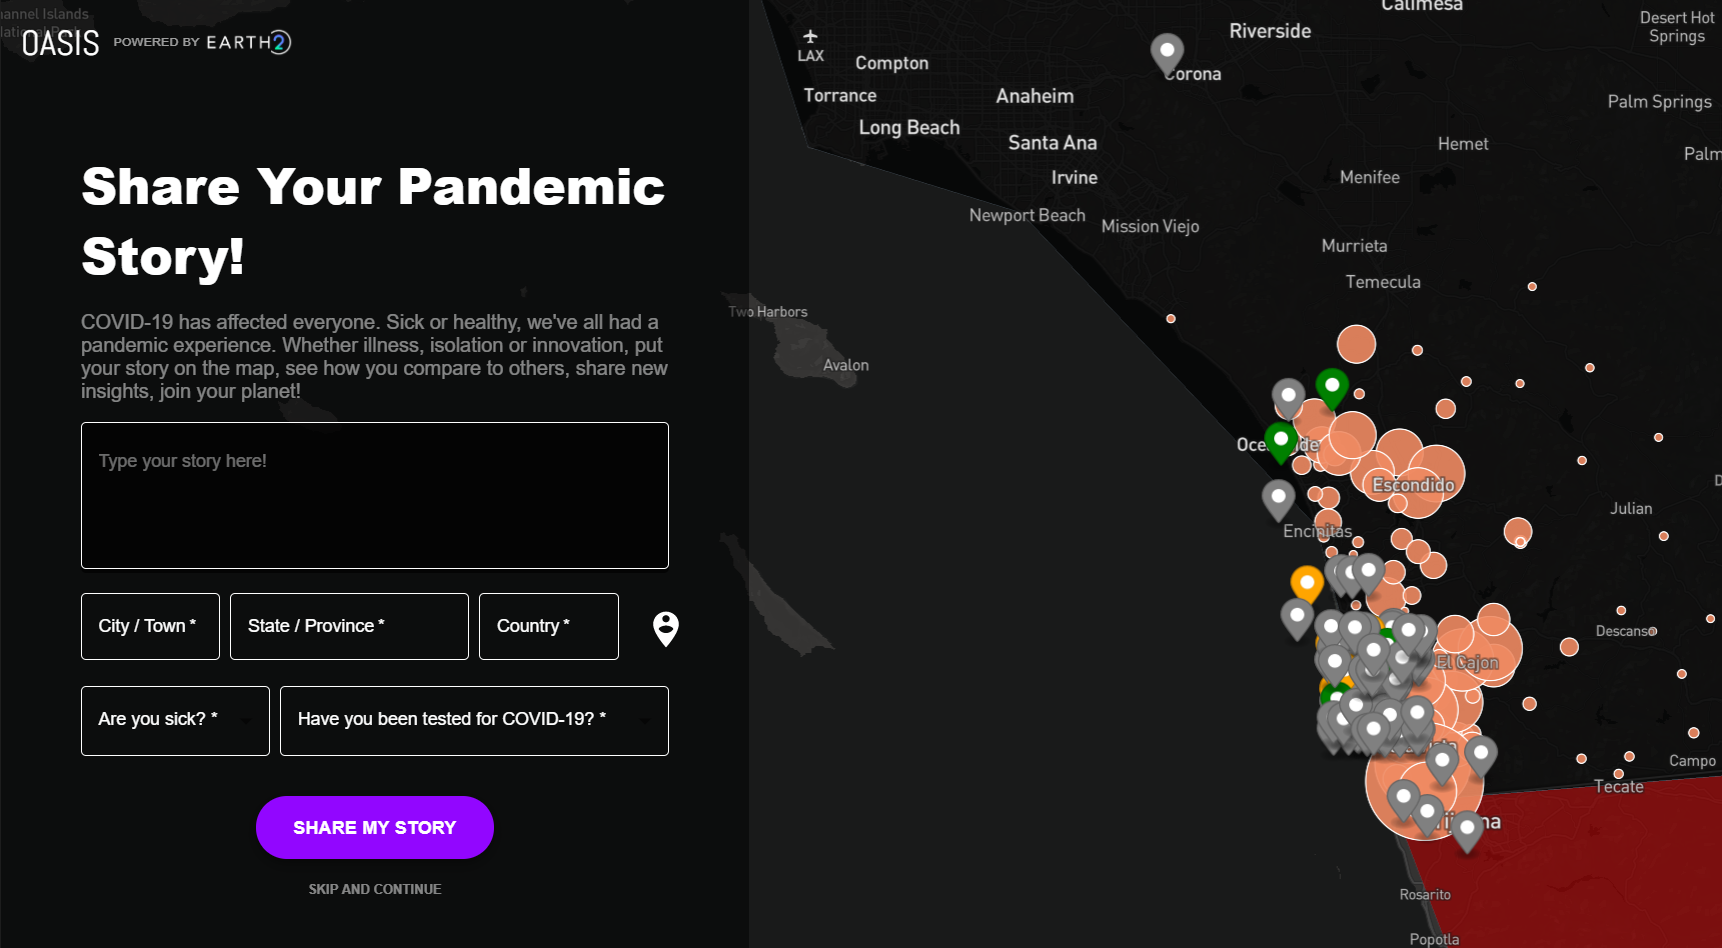
\includegraphics[scale=0.45]{images/homepage.png}
    \caption{Home Page}
\end{figure}


\subsubsection{Engagement Loop}
Even though people are willing to share their data, they do not know how they 
will benefit society or get any new information from OASIS. People go to news
websites because they want to learn about emerging events happening worldwide; 
young generations keep checking social media to see what is popular among their
peers; students go to educational websites to learn technical skills. Then, why 
would they come back to share more COVID-19 stories or update their personal
information? Other than the status of COVID-19 pandemic, OASIS must provide
its users with information that they might be interested in or do not know to
build up a long-term relationship with users.  In other words, we need to 
create an engagement loop that, on the one side, users share their data with 
OASIS, and on the other side, OASIS provides users with the insights generated
from those data. This engagement loop will generate a positive cycle, 
motivating users to share more information and enabling OASIS to get more 
diverse results from the data over and over again. 

Two main elements are involved in creating such a feedback system: natural
language processing and recommendation system. Natural language processing 
is used on mining text data, which is users’ COVID-19 stories on OASIS. It 
will generate insights that users cannot directly get from viewing other’s 
COVID-19 stories and display them on the dashboard. Recommendation systems 
will also be applied to users’ COVID-19 stories, feeding users with stories
that might interest them. By providing users more information and content 
through natural language processing and recommendation systems, OASIS is more
likely to attract more users and consolidate existing users. 

\begin{figure}[H]
    \centering
    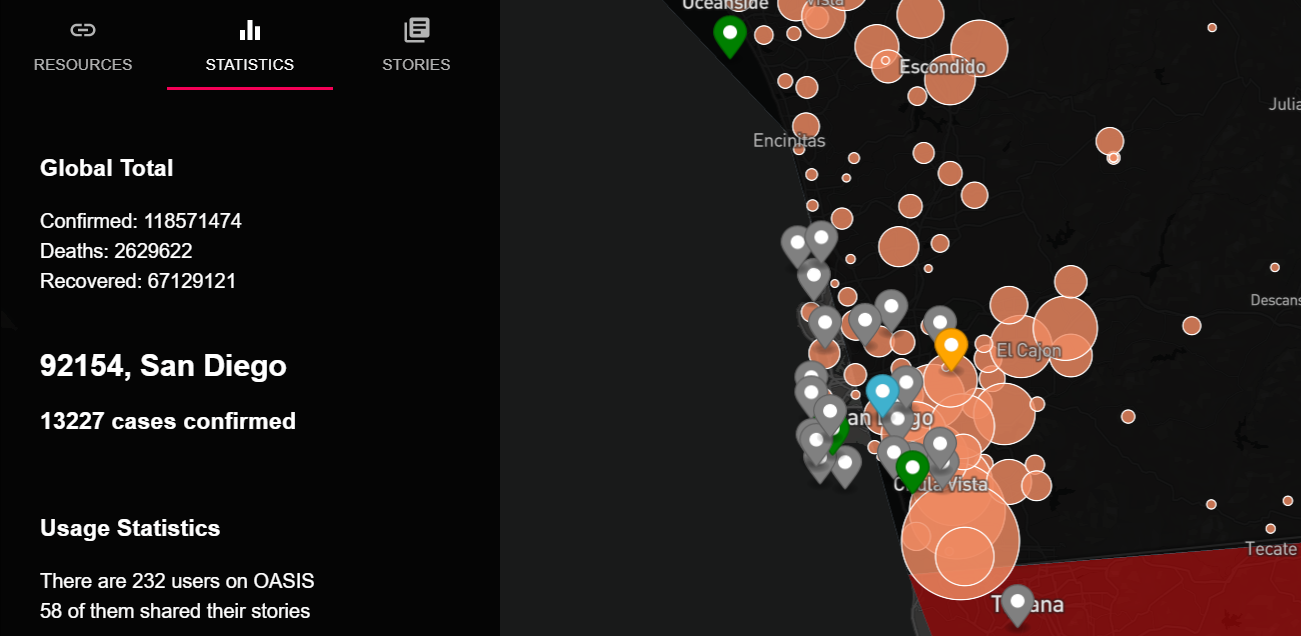
\includegraphics[scale=0.45]{images/zipcode.png}
    \caption{Zipcode Level COVID-19 Status on 3/12/2020}
\end{figure}
\begin{figure}[H]
    \centering
    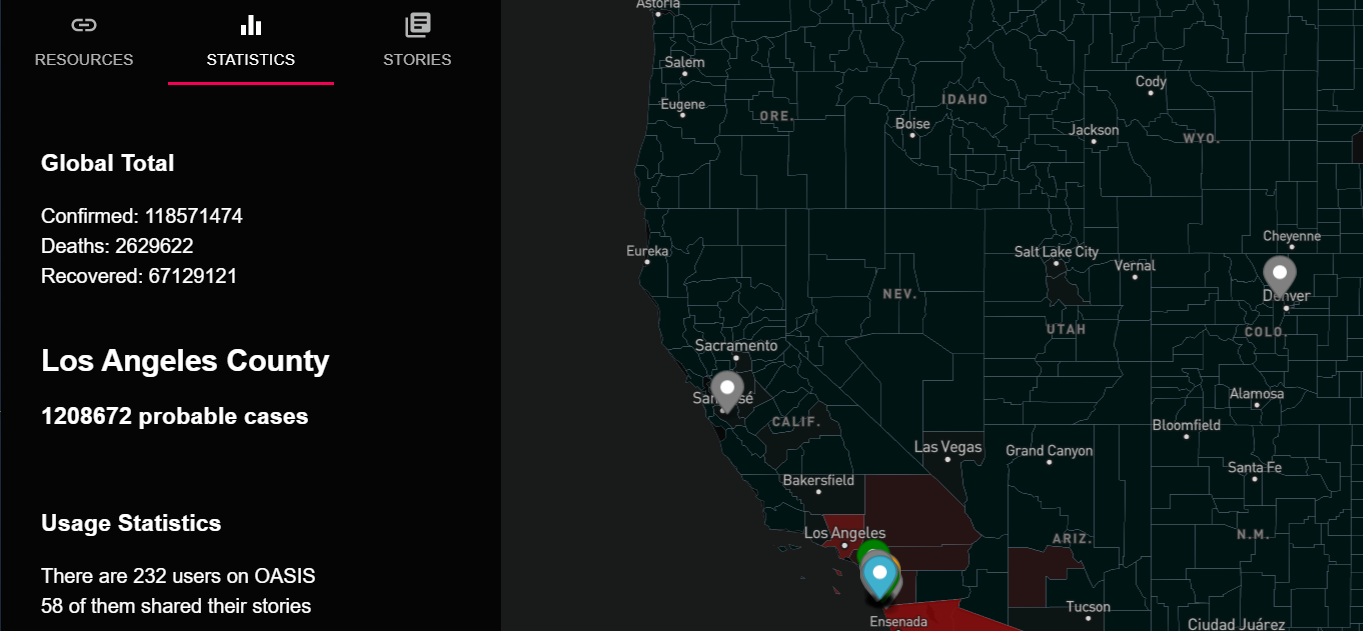
\includegraphics[scale=0.43]{images/county.png}
    \caption{County Level COVID-19 Status on 3/12/2020}
\end{figure}
\begin{figure}[H]
    \centering
    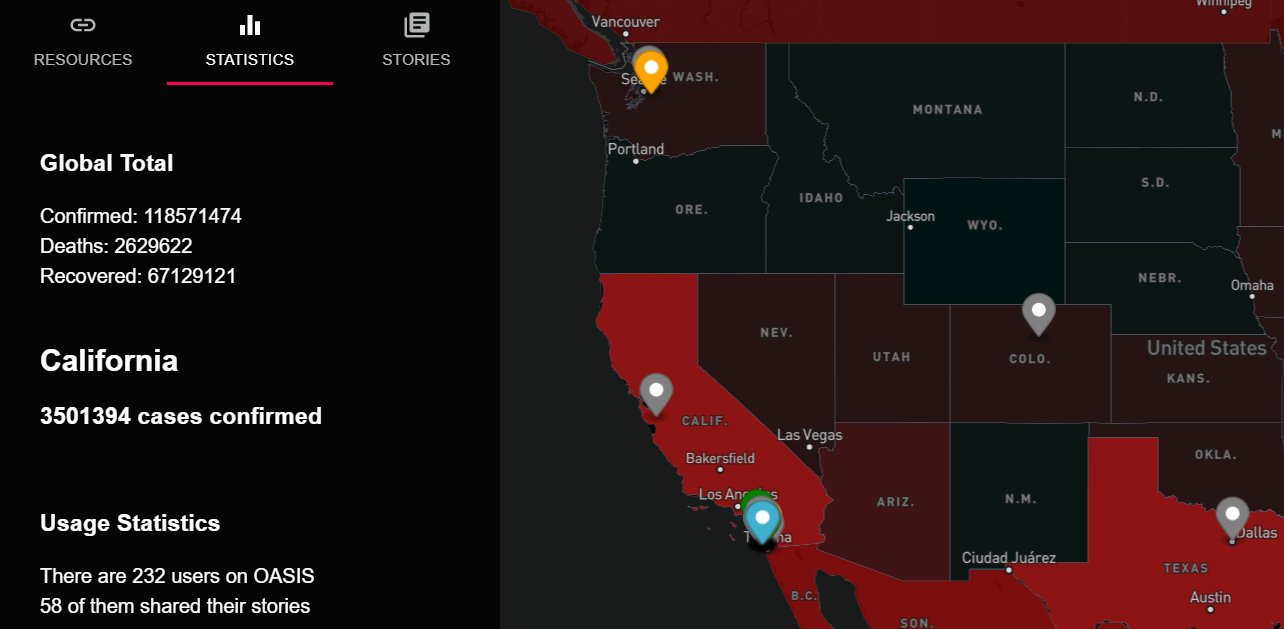
\includegraphics[scale=0.5]{images/state.png}
    \caption{State Level COVID-19 Status on 3/12/2020}
\end{figure}
\begin{figure}[H]
    \centering
    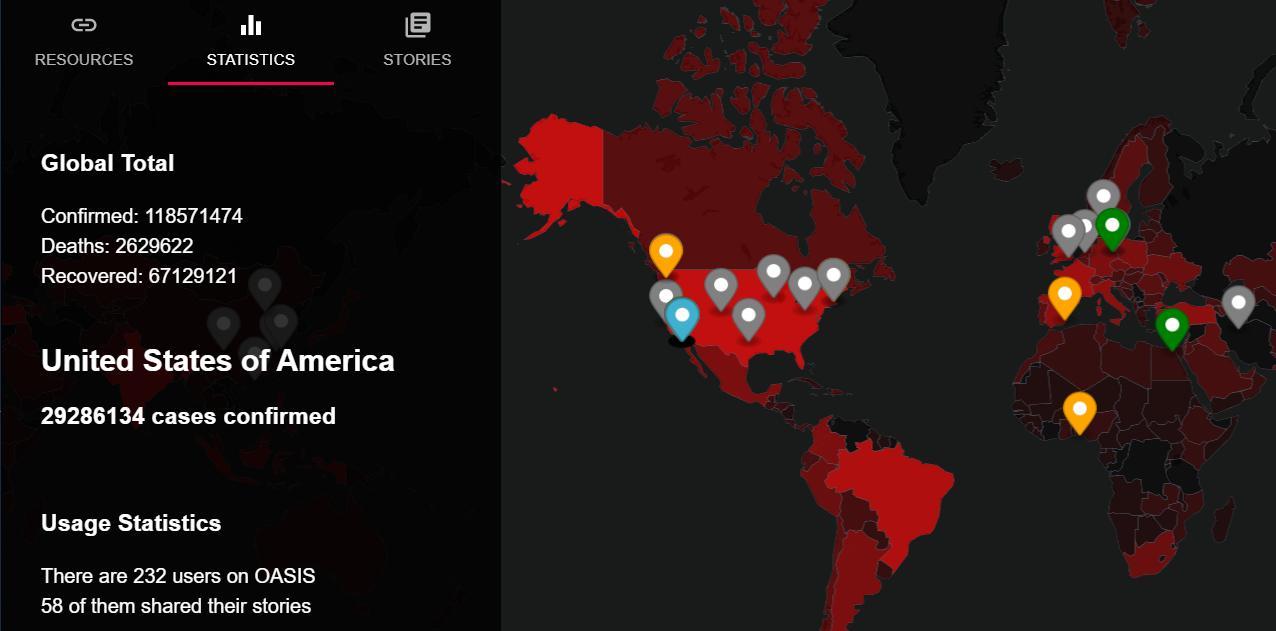
\includegraphics[scale=0.5]{images/world.png}
    \caption{World Level COVID-19 Status on 3/12/2020}
\end{figure}

\subsubsection{Natural Language Processing}
Natural Language Processing(NLP) is a subfield of artificial intelligence 
that deals with the interaction between computers and human languages. At 
OASIS, we decided to use NLP to read and decipher the users’ COVID-19 stories 
in order to generate useful information to fight against COVID-19. Several 
questions could be answered. Firstly, what is the most frequent word in the 
users’ stories? By finding out the most frequent word, we would know what 
people care the most or what affected them most during the quarantine. 
We would then know which issue we should prioritize to solve to help people 
get through and recover from the COVID-19 disaster. Secondly, what is the 
users’ attitude towards different events, like quarantine, online-learning,
and working from home, triggered by COVID-19? It might reveal the preferable
style of people’s life, work, and education. For example, if students feel
more productive during online learning, schools should consider offering
online classes to offer students better educational experiences. We can also
combine NLP with the personal information that users share on OASIS, such as 
age, gender, and professional, to get deeper insights. We might find the age
at which people are more vulnerable to getting infected. Finally, we want to
understand if we can use the same algorithm to process the data from citizens
to get insight into other natural challenges.

\begin{figure}[H]
    \centering
    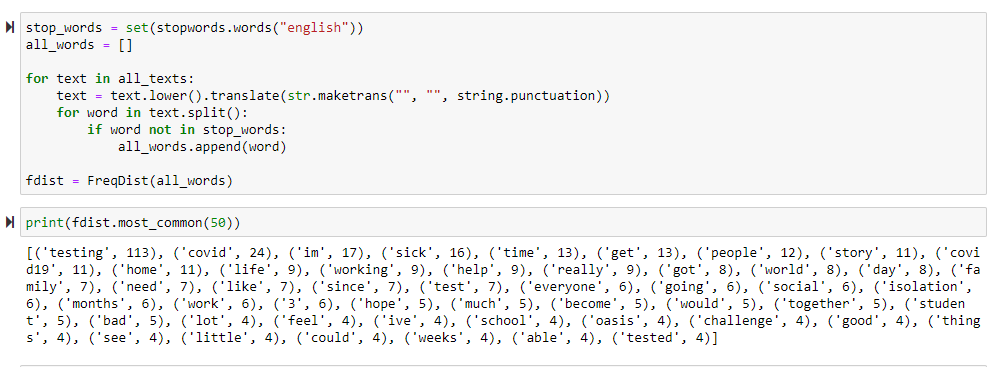
\includegraphics[scale=0.62]{images/nlp.png}
    \caption{Most Frequent Words on 3/12/2020}
\end{figure}

\subsubsection{Recommendation System}
A recommendation system is a subclass of information filtering systems that 
suggest relevant items to users. Nowadays, recommender systems are an essential
part of e-commerce and online advertisement. It can be applied to various 
applications, like Facebook, Reedit, YouTube, and LinkedIn, to attract users
by offering them what they might be interested in. 

OASIS mainly relies on content-based methods that use additional information
about users, like age, gender, professionals, locations, and medical conditions,
for the recommendation. Unlike collaborative methods based on the interaction 
between users and items, content-based methods suffer far less from the cold 
start problem than collaborative approaches (Rocca, 2019). As there are less
than 300 users in the database, content-based methods fit OASIS more. OASIS 
offers users the nearest stories based on their locations, similar stories
based on their gender, age, and professions, and popular stories among all 
the stories. 

\begin{figure}[H]
    \centering
    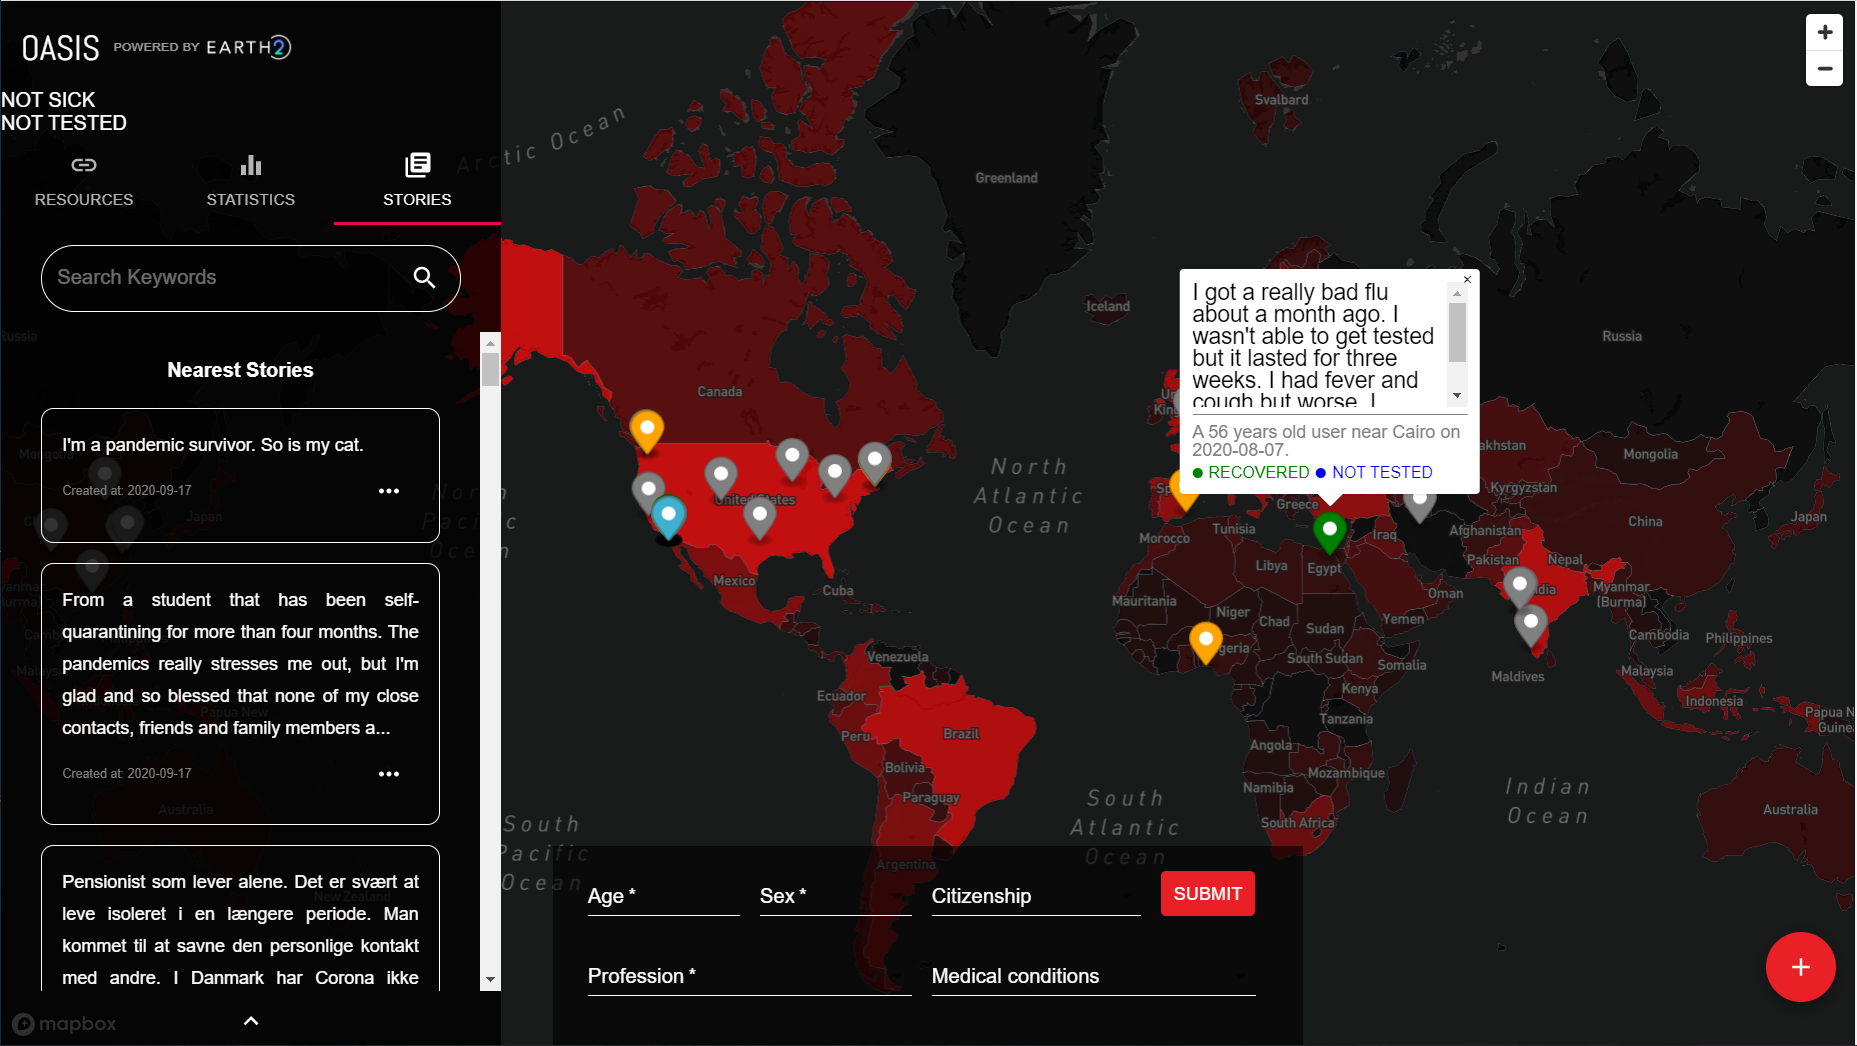
\includegraphics[scale=0.4]{images/stories.png}
    \caption{Recommended Stories}
\end{figure}


\subsubsection{Social Engagement}
Apps with a social component are typically more attractive to users than those
without. According to the most popular iPhone apps Ranking on SimilarWeb, 
out of the most 20 popular iPhone Apps in the United States in 2020, 
more than half of them have a social component. Therefore, to better promote 
OASIS among the public, this website needs to get social. There are two 
attributes to make it social: being innately social and promoting social sharing. 

Being innately social means a feature for communication, sharing, and network 
should be embedded in the apps. Therefore, besides the feature that users 
can share their stories about COVID-19 and view others’ stories on OASIS,
they should be able to like, dislike, and comment on any story. Usually, 
users share strategies to deal with the situation that the story describes, 
discuss the opinions in the story, or express their satisfaction with the
story. All these activities can improve the interaction between users and
the platform. 

To advertise OASIS, we decided to allow users to share their stories on 
other social media, such as Facebook, Instagram, and LinkedIn. People on 
those platforms get to know OASIS when they see the posts made by users on
OASIS. Besides, if anyone on those platforms replied to a particular post 
shared from OASIS, OASIS will collect its comments and store it back to the 
database, having more data for NLP and recommendation systems aforementioned. 

\begin{figure}[H]
	\begin{subfigure}{.49\textwidth}
	    \centering
		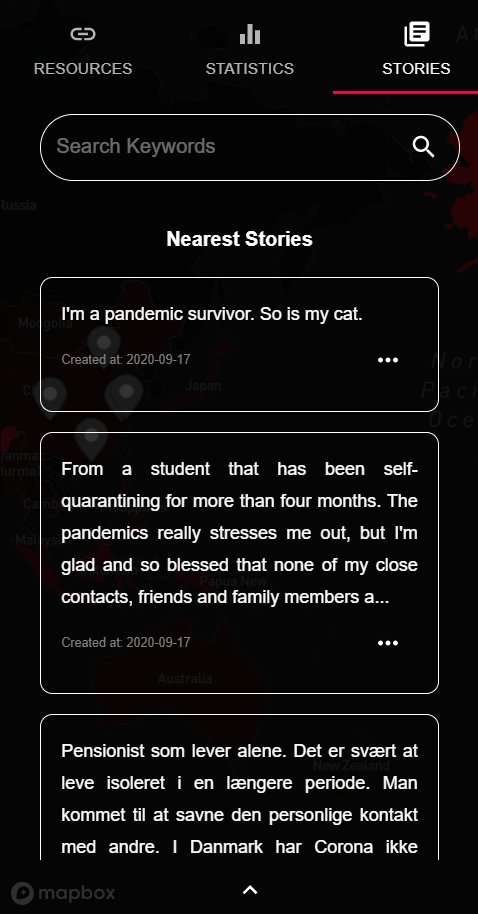
\includegraphics[scale = 0.7]{images/nearest.PNG}
	\end{subfigure}
	\begin{subfigure}{.49\textwidth}
	    \centering
		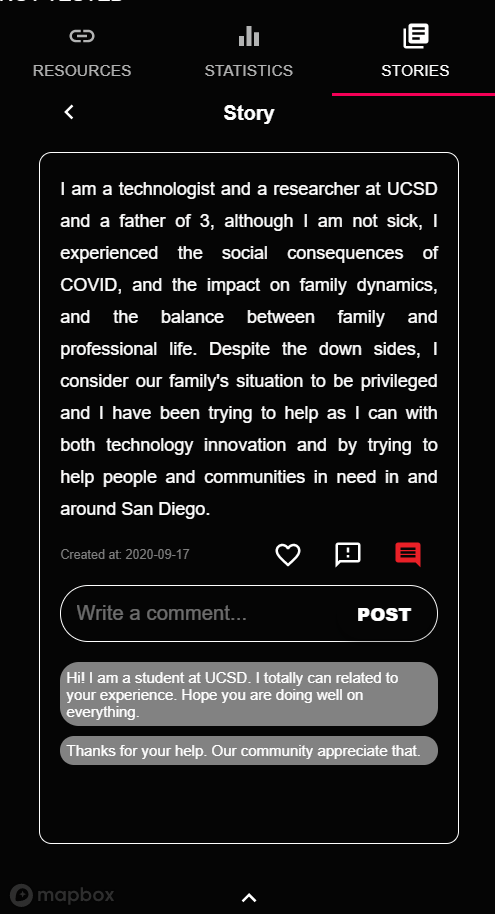
\includegraphics[scale = 0.7]{images/comments.PNG}
	\end{subfigure}
	\caption{Nearest Stories and Comments}
\end{figure}


%%%%%%%%%%%%%%%%%%%%%%%%%%%%%%%%%%%%%%%%%%%%%%%%%%%%%%%%%%%%%%%%%%%%%%%%%%%%%%%
\subsection{Privacy Concern}
Recall the most significant issue in COVID Maps: users are unwilling to share 
their data due to privacy concerns. Therefore, for OASIS, we need to make sure:

\begin{enumerate}
    \item Avoid getting access to the private informations on user’s Google account,
    \item Avoid storing geodata on the server.
    \item Keep geodata at all times disassociated from personally identifiable 
    information: while data is in transit, in memory, and so on, we need to make
    sure it cannot be associated with the user.
\end{enumerate}

Firstly, OASIS allows users to “continue as a guest,” allowing anonymous 
sign-in. Instead of email and password combination, it creates a cookie for 
identification, which gets expired after five days. To balance privacy and data
collection, we require every user to input their city, province, country, test
status, and stories about COVID-19. If they do
not fill in those pieces of information on the home page but clicks on “skip and
continue,” which directs them to the sign-in page, they have to redirect to the
home page and share those pieces of information.

 
Secondly, we gave up on GPS history sharing. We require users to input their 
country, city, province, and country to put their stories on the map. However,
we do not store any geodata, like coordinates, anymore. 

Thirdly, we avoid the association between the user’s identification email and 
geographical data. Since the email address is the only way to identify the 
user, OASIS API calls do not return the user’s email address and the
geographical information simultaneously. Also, we randomize the markers on the
map to avoid associating a user with a particular place.

\begin{figure}[H]
    \centering
    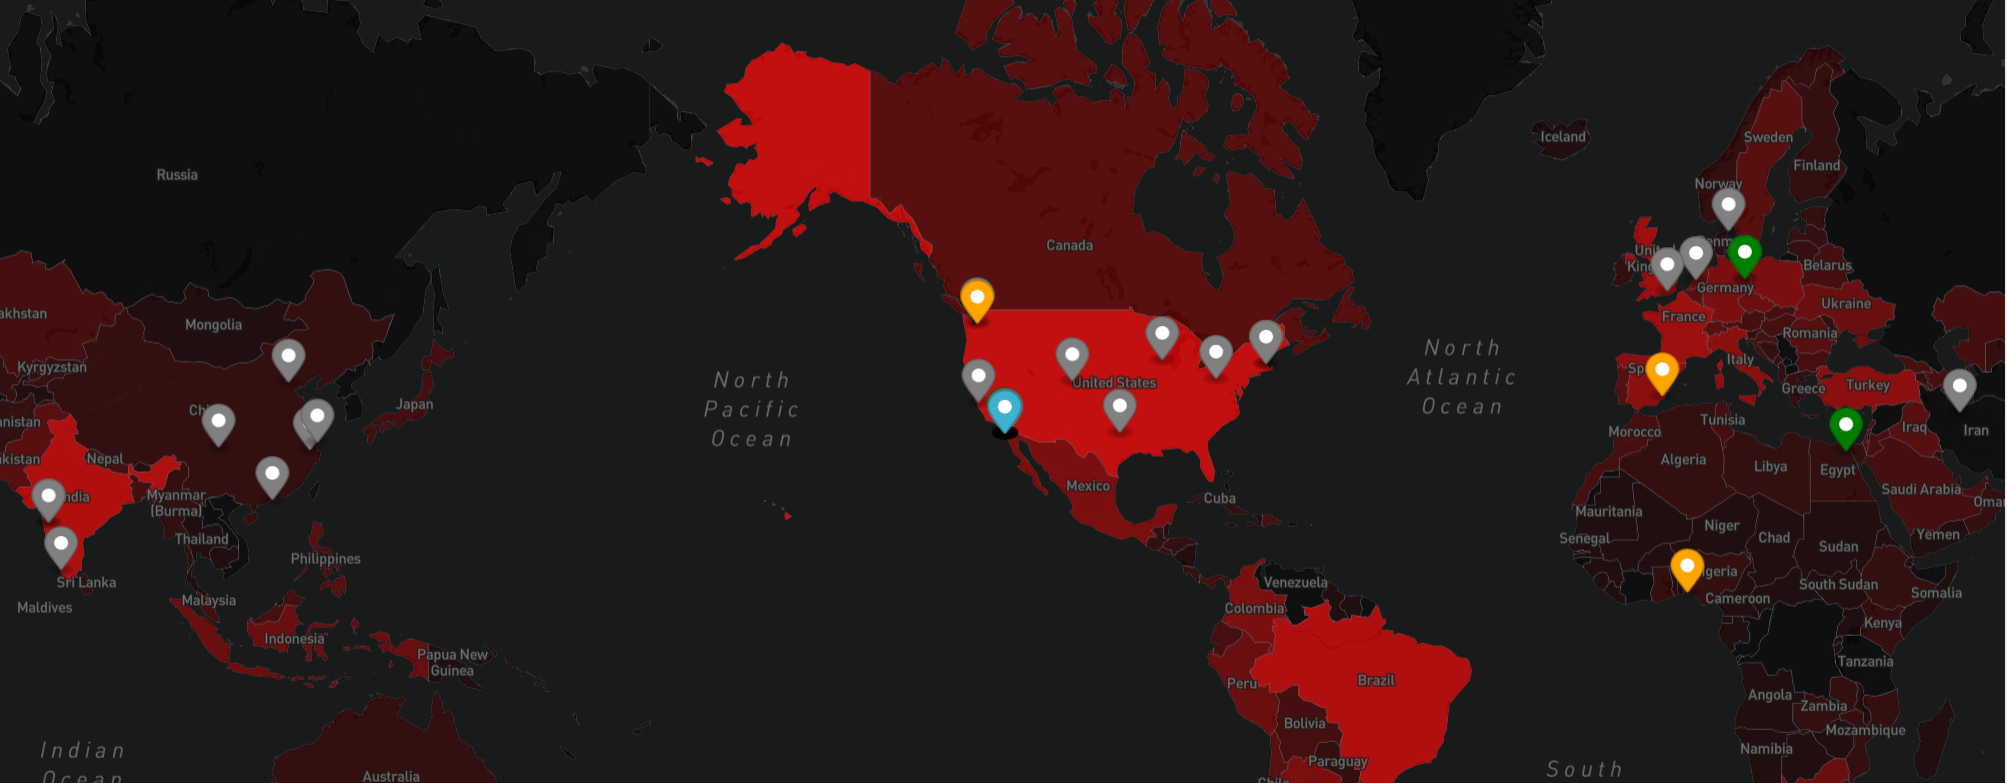
\includegraphics[scale=0.38]{images/markers.png}
    \caption{Randomized Markers}
\end{figure}


%%%%%%%%%%%%%%%%%%%%%%%%%%%%%%%%%%%%%%%%%%%%%%%%%%%%%%%%%%%%%%%%%%%%%%%%%%%%%%%
\subsection{Development and Toolbox}
We used React JS to develop the front-end of OASIS. We also used Redux for 
application status management. For data visualization on the user side, we 
applied Mapbox to build the map for COVID-19 cases and user story display. 

On the back-end, we chose Python and MySQL for the database systems. Flask 
allows us to quickly create a ReST API and provide the front-end with safe 
function calls to the database. To better manage the database’s version, we 
utilized alembic for data migration. 

To integrate different stacks, we used Github project management for task
assignment and code review. We also dockerized the local development environment
for testing. Besides human testing, we applied Travis on GitHub to do automated
testing, avoiding branch conflict and API function call bugs. 

Finally, we applied AWS for the server and Rancher to run containers in 
production. Now, we are trying to migrate everything to Heroku for simple usage. 

\begin{figure}[H]
    \centering
    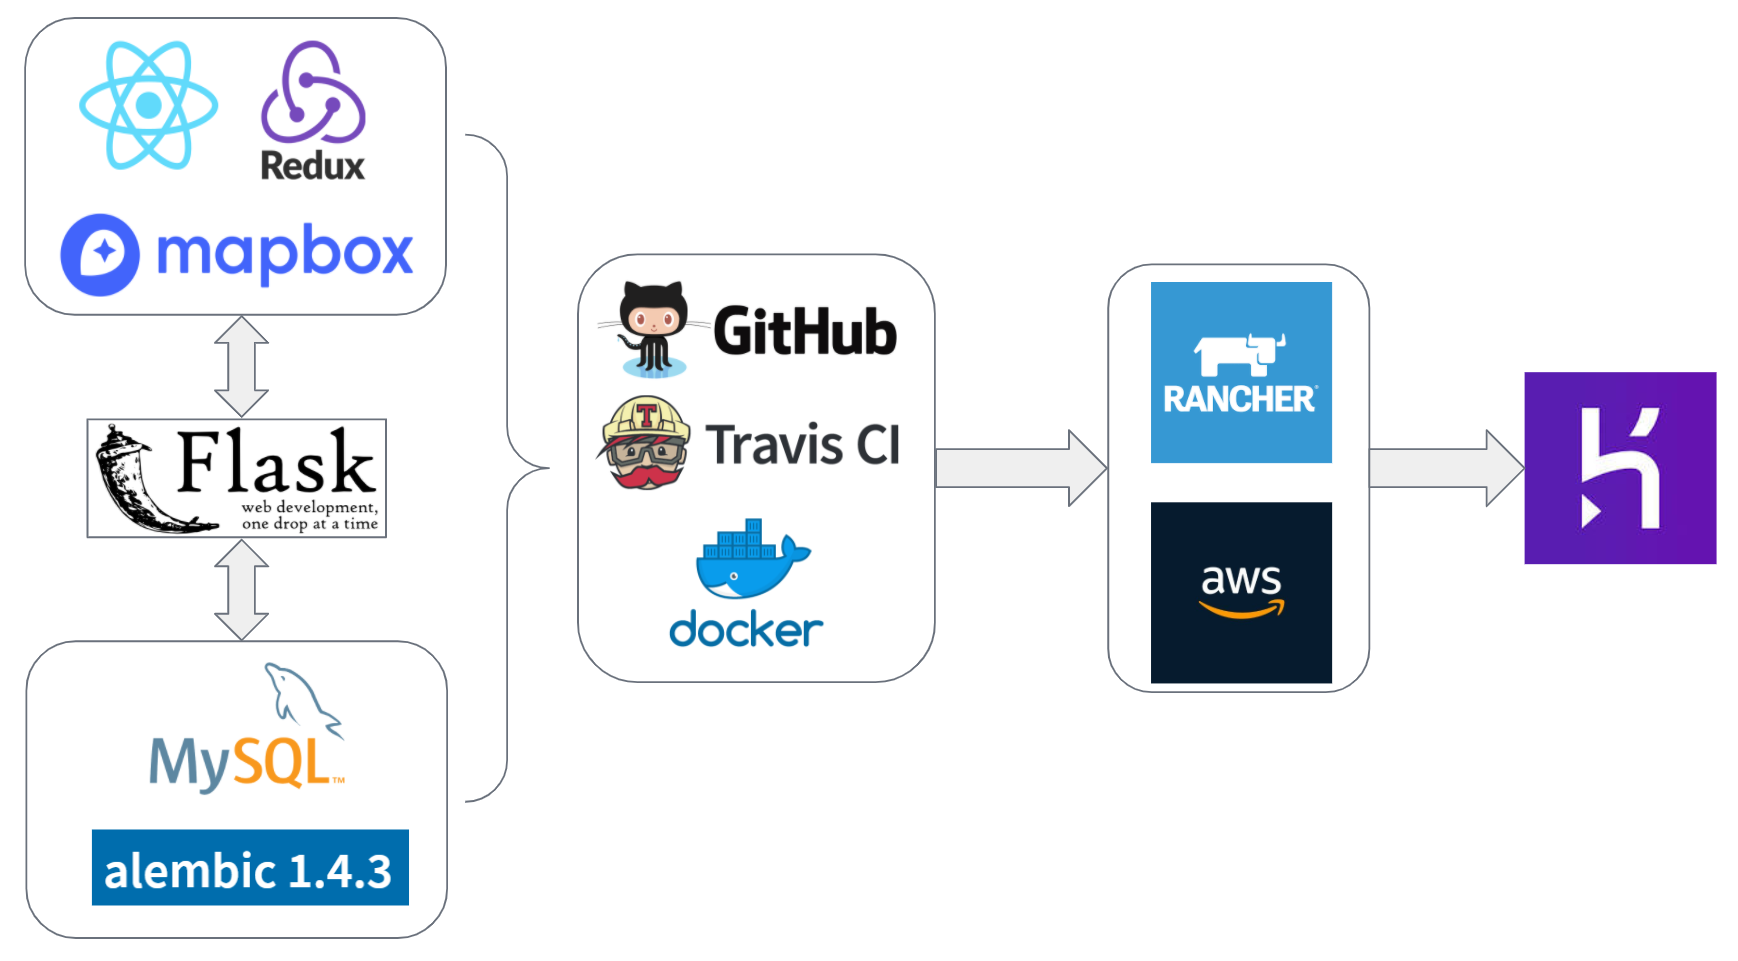
\includegraphics[scale=0.4]{images/tools.PNG}
    \caption{Toolbox}
\end{figure}

%%%%%%%%%%%%%%%%%%%%%%%%%%%%%%%%%%%%%%%%%%%%%%%%%%%%%%%%%%%%%%%%%%%%%%%%%%%%%%%
\subsection{Result}
The OASIS team started to build the platform in June 2020, trying to simplify
the process of data sharing and processing. After 6 month’s work, OASIS has the 
following linear user flow:

\begin{figure}[H]
    \centering
    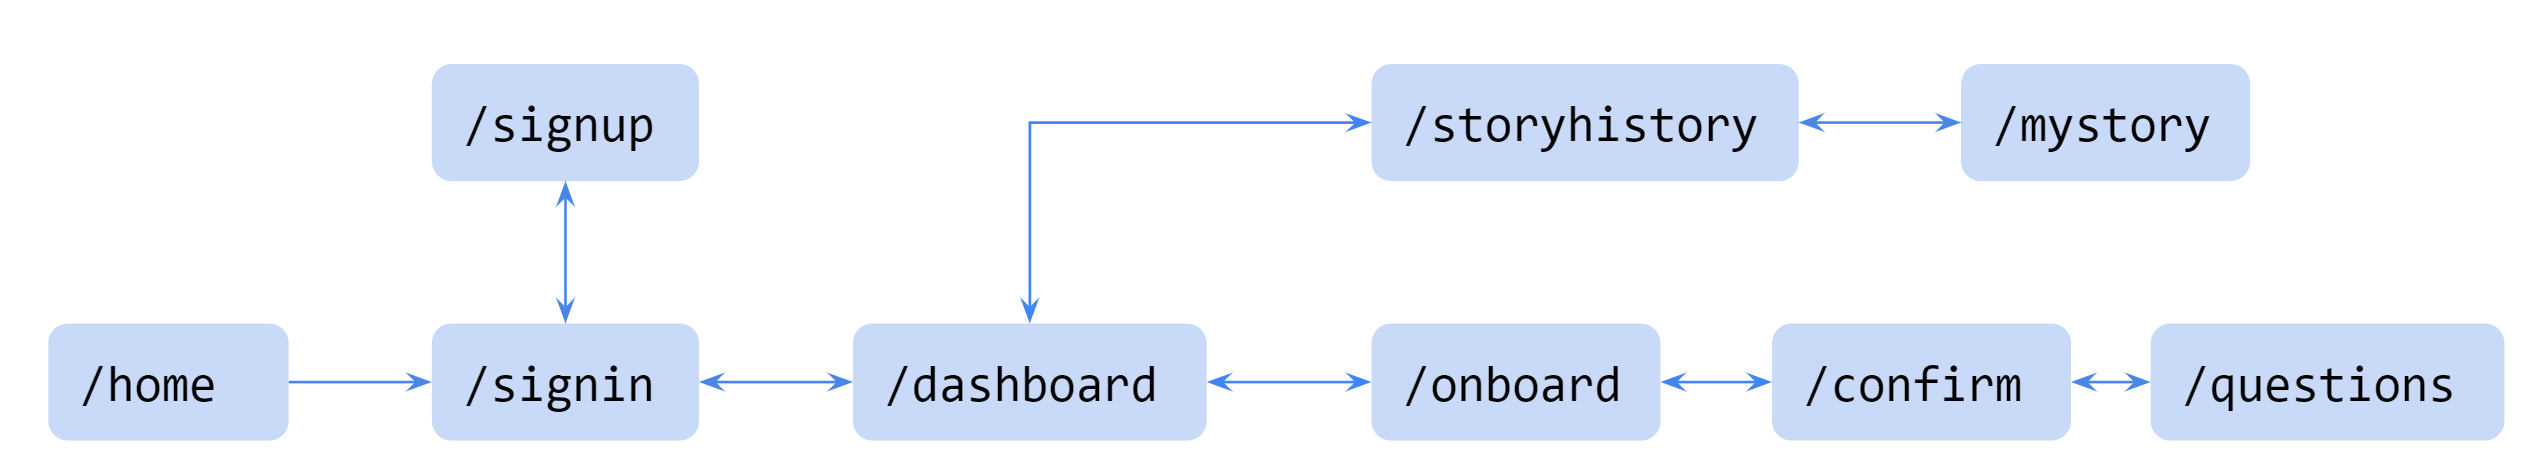
\includegraphics[scale=0.3]{images/userflow.png}
    \caption{User Flow}
\end{figure}


Users share their COVID-19 story, location, and test status on the home page,
or choose “skip and continue” to directly go to the sign-in page. However, if
the current user does not have an account and has not shared a story, they must
go back to the home to their such personal information first. The user can then
create an account through the sign-up page and redirect back to the sign-in 
page. In other words, users must at least share their  COVID-19 story, 
location, and test status in order to get the information and service provided
in the dashboard. 


In the dashboard, users can get confirmed cases of COVID-19 in different 
regions from the country level to zip code level. They can also view, search,
and comment on other users’ stories and get recommended stories from the system.
They also can get trustable resources for dealing with COVID-19. Through the
/storyhistory to /mystory chain, users can share their own COVID-19 stories. 
Through the /onboard, /confirm, to /questions chain, users can share or update 
their personal information, including age, sex, citizenship, professions, and
medical conditions. 

\begin{figure}[H]
	\begin{subfigure}{.33\textwidth}
	    \centering
		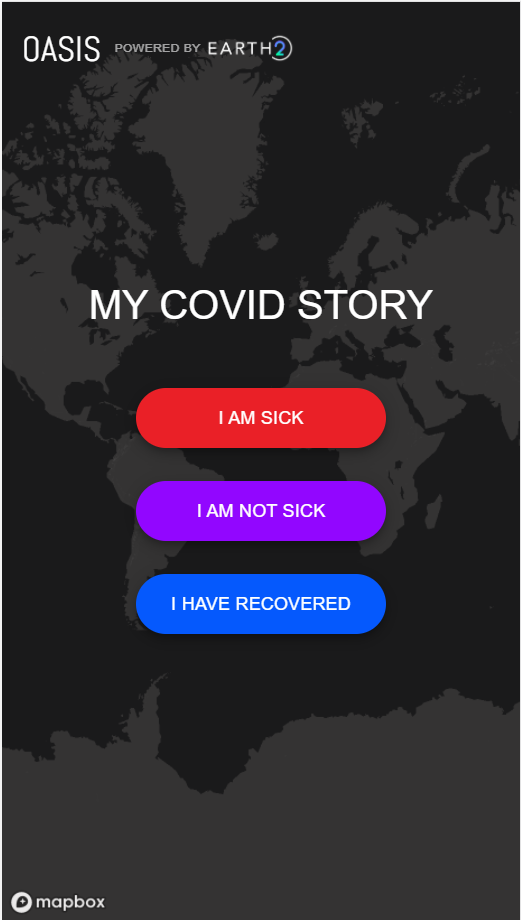
\includegraphics[scale = 0.47]{images/update1.PNG}
		\caption{/onboard}
	\end{subfigure}
	\begin{subfigure}{.33\textwidth}
	    \centering
		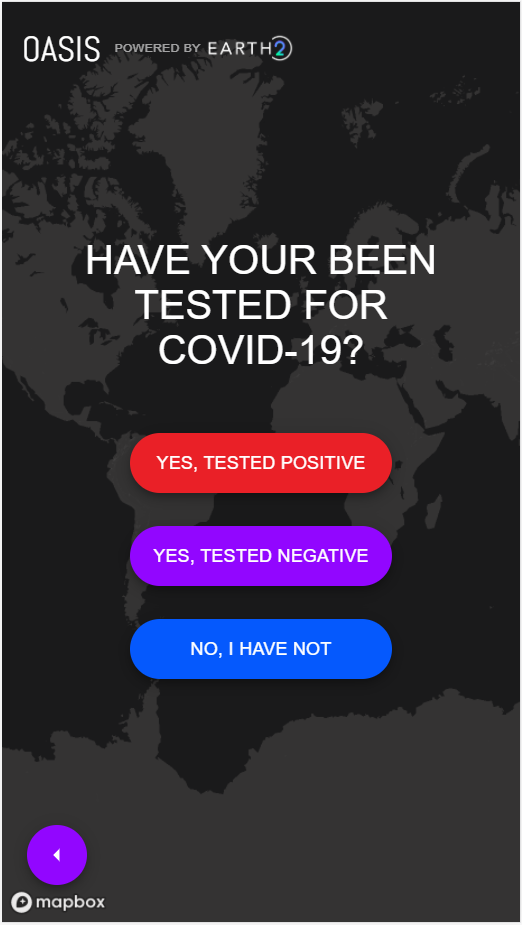
\includegraphics[scale = 0.47]{images/update2.PNG}
		\caption{/confirm}
	\end{subfigure}
	\begin{subfigure}{.33\textwidth}
	    \centering
		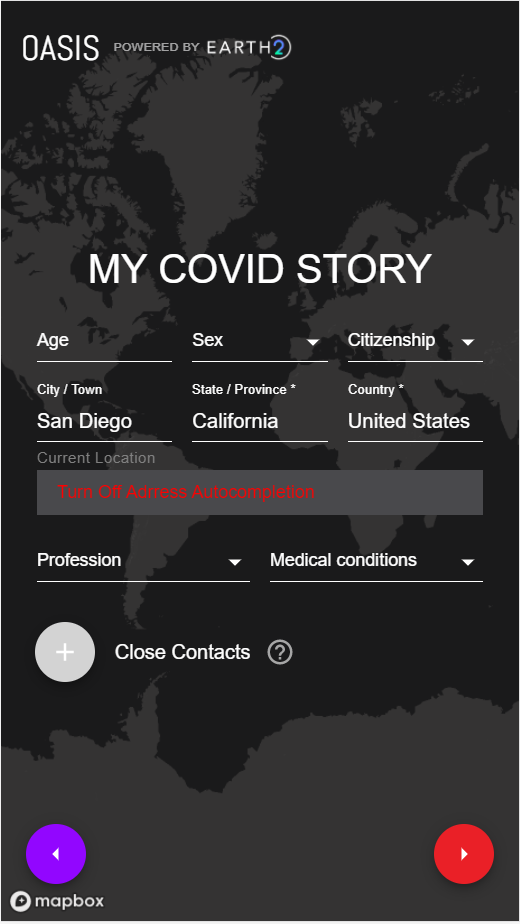
\includegraphics[scale = 0.47]{images/update3.PNG}
		\caption{/question}
	\end{subfigure}
	\caption{ Mobile View of Updating User Profile}
\end{figure}

\begin{figure}[H]
	\begin{subfigure}{.33\textwidth}
	    \centering
		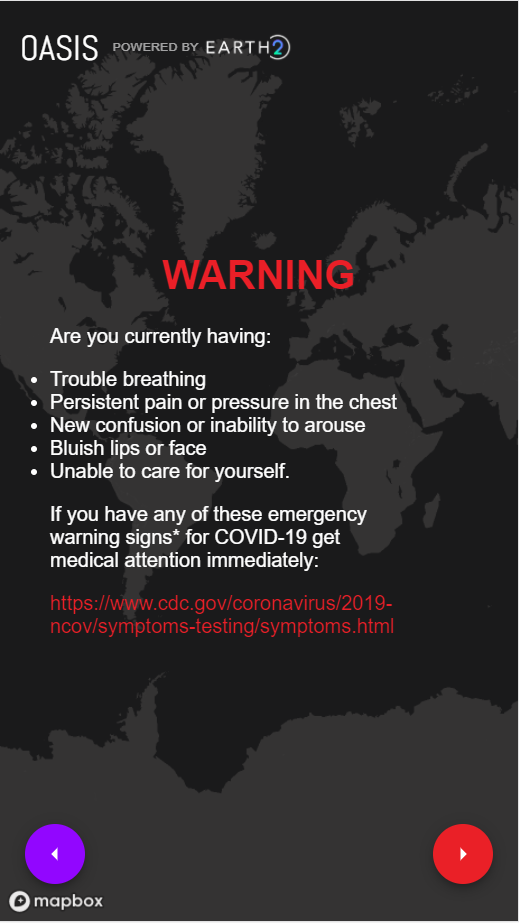
\includegraphics[scale = 0.47]{images/update4.PNG}
		\caption{/onboard}
	\end{subfigure}
	\begin{subfigure}{.33\textwidth}
	    \centering
		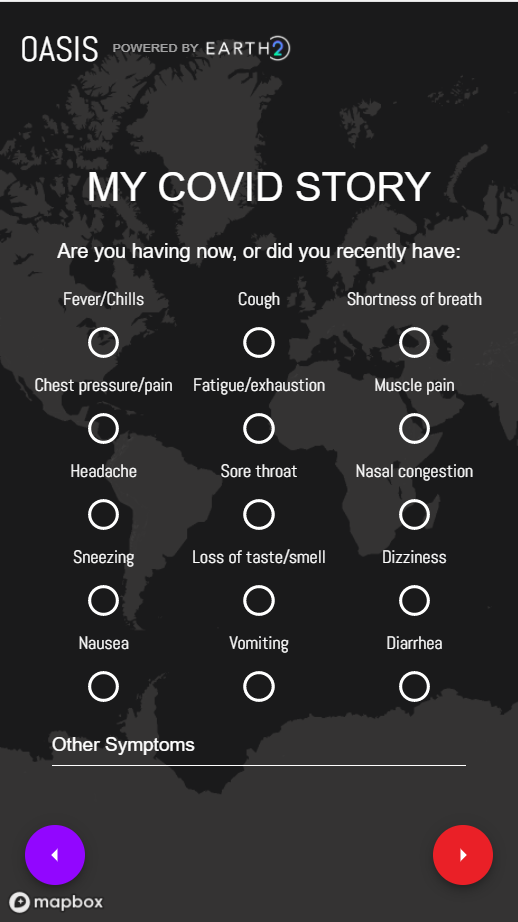
\includegraphics[scale = 0.47]{images/update5.PNG}
		\caption{/confirm}
	\end{subfigure}
	\begin{subfigure}{.33\textwidth}
	    \centering
		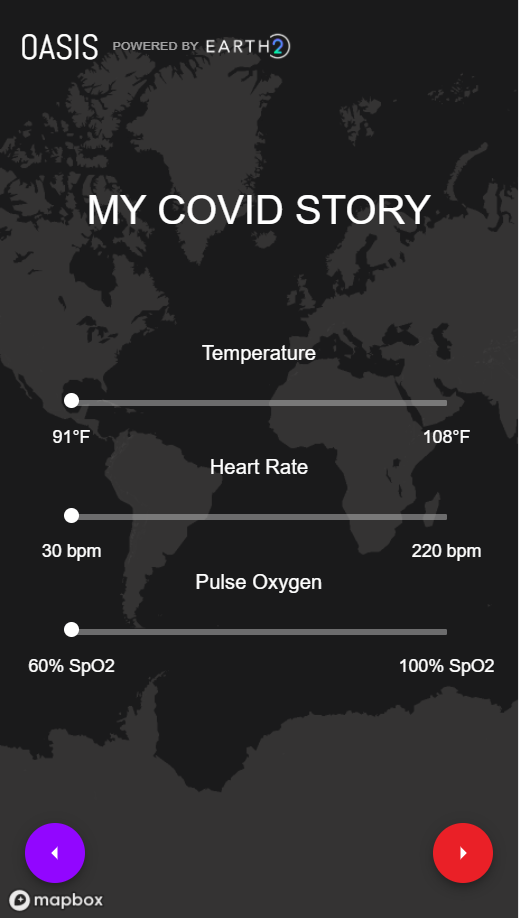
\includegraphics[scale = 0.47]{images/update6.PNG}
		\caption{/question}
	\end{subfigure}
	\caption{Input Health Status If Input Tested Positive}
\end{figure}


\begin{figure}[H]
    \centering
    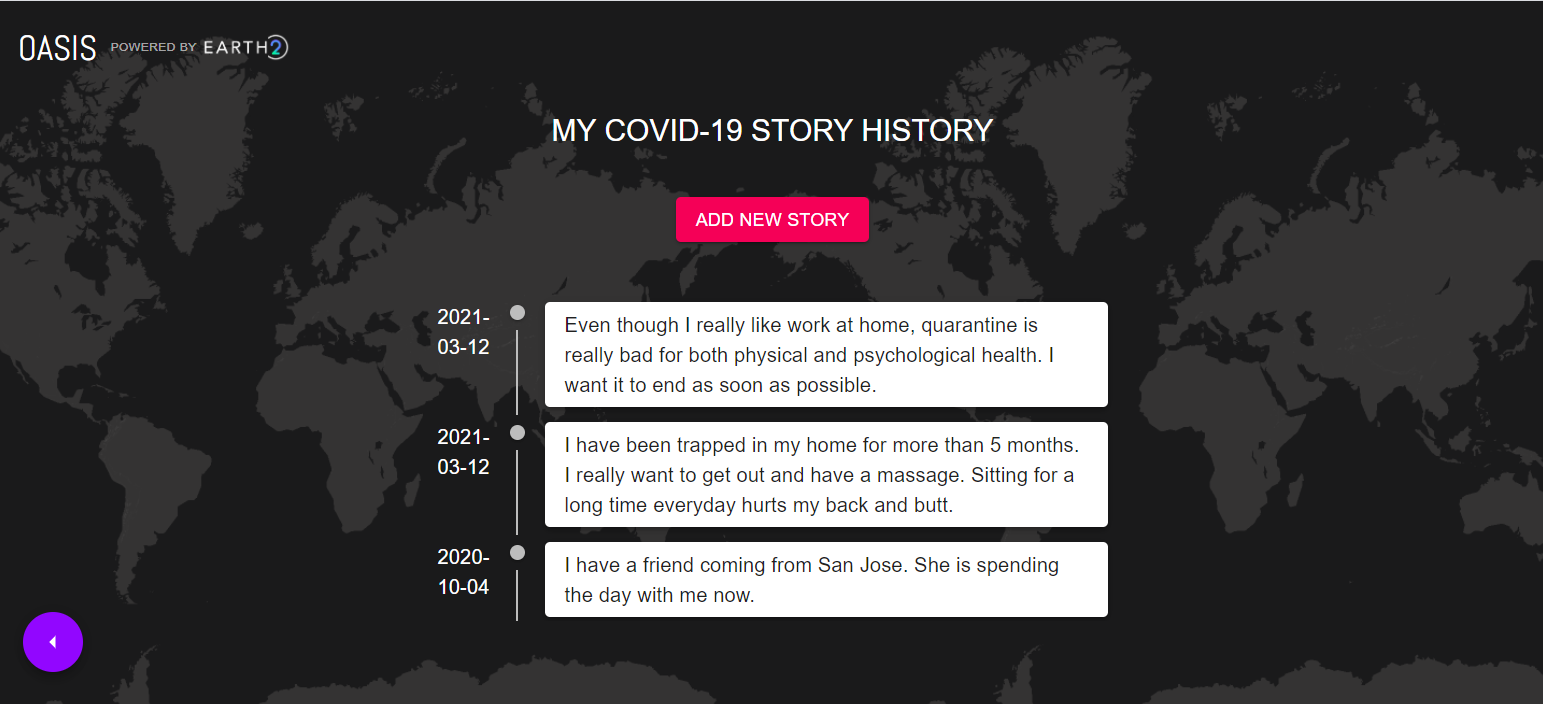
\includegraphics[scale=0.5]{images/mystories.PNG}
    \caption{Share COVID-19 Stories}
\end{figure}



Until 01/27/2020, OASIS has attracted about 230 users. Most of them come from 
America, China, Indian, Singapore, and Europe. About half of them are between 
18 and 34 years old. Finally, about 45\% of them are female, and 55\% are
male. The following charts are data from Google Analytics since September 2020.


\begin{figure}[H]
	\centering
	\begin{subfigure}{.49\textwidth}
		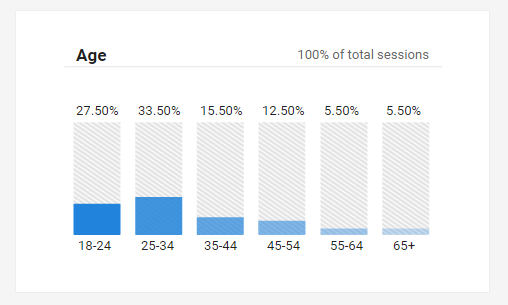
\includegraphics[scale = 0.75]{images/age.PNG}
		\caption{Ages}
	\end{subfigure}
	\begin{subfigure}{.49\textwidth}
		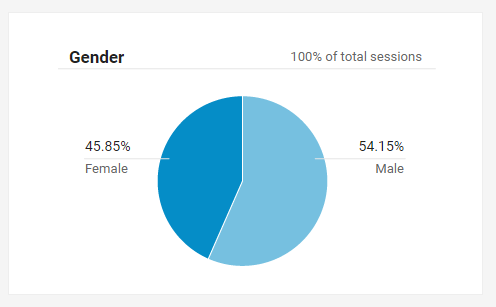
\includegraphics[scale = 0.75]{images/geneder.PNG}
		\caption{Genders}
	\end{subfigure}
	\caption{Data from Google Analytics Since September 2020}
\end{figure}


\newpage
%%%%%%%%%%%%%%%%%%%%%%%%%%%%%%%%%%%%%%%%%%%%%%%%%%%%%%%%%%%%%%%%%%%%%%%%%%%%%%%
%%%%%%%%%%%%%%%%%%%%%%%%%%%%%%%%%%%%%%%%%%%%%%%%%%%%%%%%%%%%%%%%%%%%%%%%%%%%%%%
%%%%%%%%%%%%%%%%%%%%%%%%%%%%%%%%%%%%%%%%%%%%%%%%%%%%%%%%%%%%%%%%%%%%%%%%%%%%%%%
\section{Conclusion}

%%%%%%%%%%%%%%%%%%%%%%%%%%%%%%%%%%%%%%%%%%%%%%%%%%%%%%%%%%%%%%%%%%%%%%%%%%%%%%%
%%%%%%%%%%%%%%%%%%%%%%%%%%%%%%%%%%%%%%%%%%%%%%%%%%%%%%%%%%%%%%%%%%%%%%%%%%%%%%%
\subsection{Summary}
To fight against COVID-19, Professor Henrik I. Christensen and I proposed 
COVID Maps. We designed a website that allows users to share their GPS location
histories from Google Maps Timeline and inform the hotpots of COVID‑19 
transmission. In this project, I was the programmer and designer to achieve 
the following three functionalities through JavaScript, HTML, Bootstrap, and 
Firease:
\begin{enumerate}
    \item It parses the shared GPS data from KML files into GEOJSON objects.
    \item It stores the data in a tree structure for further efficient usage.
    \item It informs users of the occupancy and intersectionality of a city 
    by Mapbox based on the GPS data that they provided.
\end{enumerate}

Later, we created OASIS to address privacy concerns discovered through COVID 
Maps. It creates an online platform where users can:
\begin{enumerate}
    \item view up‑to‑date COVID‑19 cases from country level to zip code level
    \item get personalized resources for dealing with COVID‑19
    \item share their stories about COVID‑19 and view, search, comment on other
    users' stories
\end{enumerate}
In  this project,  I led a 7‑person research team composed of graduate 
students, undergraduate students, and professors in agile development and 
deployment based on Travis, Docker, AWS, and Rancher. As a team leader,
I held weekly stand‑up meetings, coordinated with the third‑party company
InSTEDD for early‑stage development and deployment, helped teammates with
technical challenges, delegated tasks through GitHub project management, and
assured the quality of team deliveries. As the main programmer, I visualized
data by React, Python, MySQL, and Mapbox, conducting code reviews on GitHub, 
and testing in local and production environments. Even though we delivered
many features of OASIS, it still faces the challenge of attracting users. 


\begin{figure}[H]
    \centering
    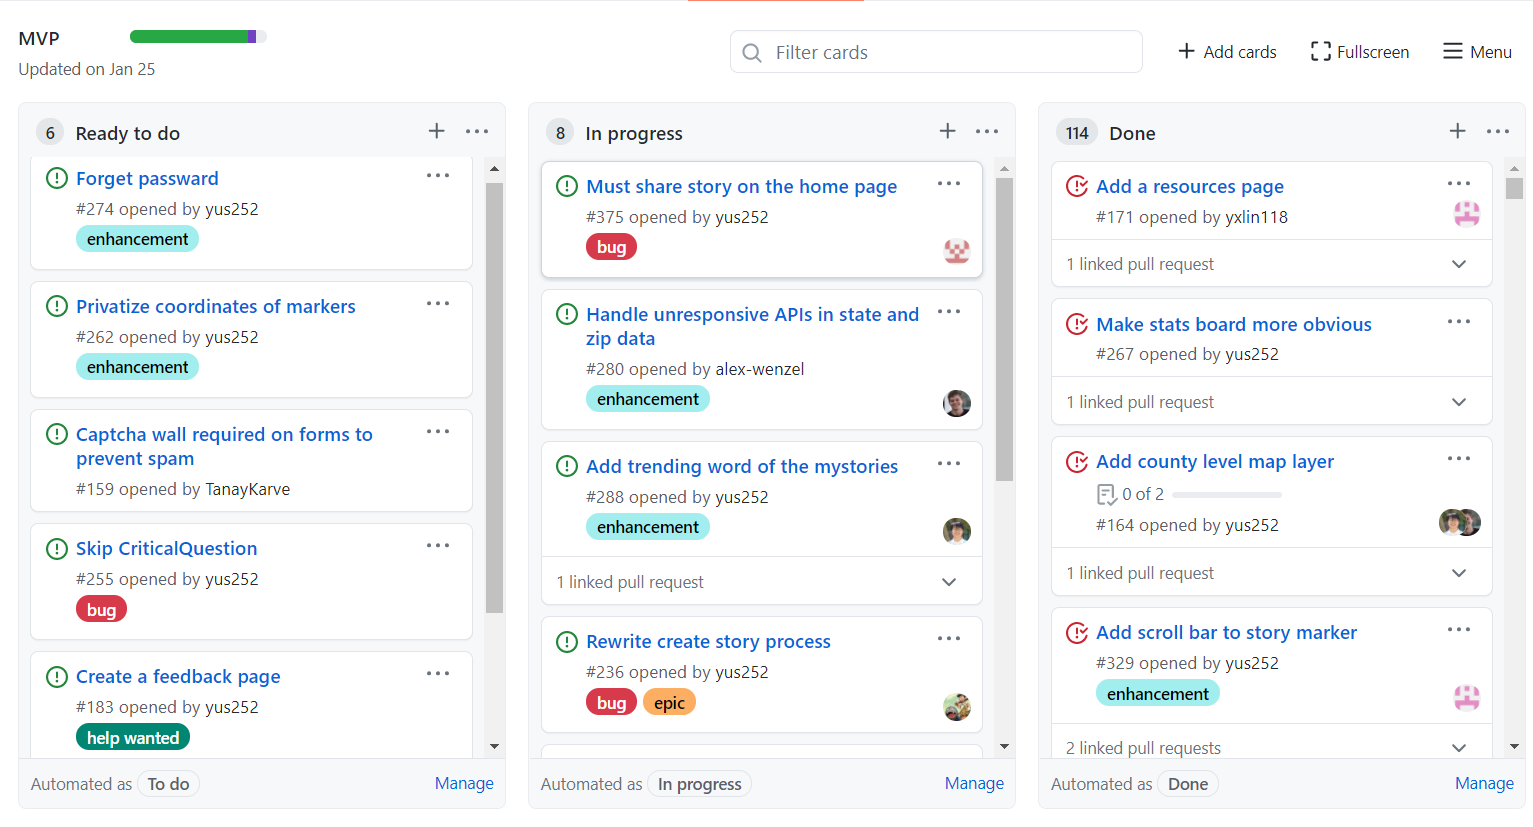
\includegraphics[scale=0.5]{images/management.png}
    \caption{Project Management on GitHub}
\end{figure}


%%%%%%%%%%%%%%%%%%%%%%%%%%%%%%%%%%%%%%%%%%%%%%%%%%%%%%%%%%%%%%%%%%%%%%%%%%%%%%%
%%%%%%%%%%%%%%%%%%%%%%%%%%%%%%%%%%%%%%%%%%%%%%%%%%%%%%%%%%%%%%%%%%%%%%%%%%%%%%%
\subsection{Lessons and Outlooks}

Firstly, through COVID Maps, we learned that privacy safety is users' most 
significant concern on every application. An IBM study found that 81\% of 
consumers say they have become more concerned about how their data is used
online (Chakravorti, 2020). One solution is legislative fixes, such as 
Europe's General Data Protection Regulation (GDPR), providing rigorous rules
about collecting and using personal data. 
However, under particular circumstances, such as the
COVID-19 pandemic, we might need more flexibility about data collection and 
usage. Is there any other way to address users' privacy concerns instead of 
avoiding collecting data? Computer security scientists might view this question
as "how to protect users' data," which is a big question. One aspect to 
consider is how we can process users' data to get insights without storing 
their data, retrieve the insights later on, and update them with the newly
collected data?

Secondly, through OASIS, we learned that to build a citizen-centric 
infrastructure, we need to simplify the process for sign up but multiple
features for people to interact with. In both OASIS and COVID Maps, users 
gave up on sharing their data because the data sharing process is 
complicated. Therefore, at OASIS, we tried to minimize the number of clicks 
users have to complete the data sharing (“fill my information”) process. 
Such an infrastructure should “reward” users for their data sharing as soon 
as possible to attract their attention by allowing users to enter the 
dashboard quickly. Next, in the dashboard, users should interact with multiple
features, just like viewing COVID-19 statistics, checking out other people’s
COVID-19 stories, getting the trending words, and recommended stories on
OASIS. 

Finally, the open question is, “can we build up a centralized database or
data-sharing platform that the public can trust in?” During the COVID-19
pandemic in the U.S., governments and some local citizen-centric 
organizations published contact tracing apps or resource sharing platforms. 
As a result, people were directed to different platforms. Each of the 
platforms has much fewer users. Since there is no connection between them,
they failed to share resources and information, not able to generating insights
through artificial intelligence. Therefore, how can we connect citizens, 
experts, governments, NGOs, and industry to solve a single issue? Or is there 
any other way to solve resource/data distribution?


%%%%%%%%%%%%%%%%%%%%%%%%%%%%%%%%%%%%%%%%%%%%%%%%%%%%%%%%%%%%%%%%%%%%%%%%%%%%%%%
%%%%%%%%%%%%%%%%%%%%%%%%%%%%%%%%%%%%%%%%%%%%%%%%%%%%%%%%%%%%%%%%%%%%%%%%%%%%%%%
%%%%%%%%%%%%%%%%%%%%%%%%%%%%%%%%%%%%%%%%%%%%%%%%%%%%%%%%%%%%%%%%%%%%%%%%%%%%%%%
\newpage
\section{Appendix}
\subsection{The Haversine Formula in JavaScript}
\href{https://www.movable-type.co.uk/scripts/latlong.html}
{\color{blue}{Calculate distance, bearing and more between Latitude/Longitude points (Veness 2019)}}
\begin{figure}[H]
    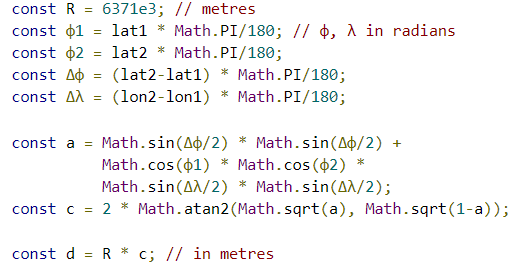
\includegraphics[scale=0.85]{images/haversine.PNG}
\end{figure}

\subsection{The General Data Protection Regulation}
\href{https://en.wikipedia.org/wiki/General_Data_Protection_Regulation}
{\color{blue}{From Wikipedia:} } \\
The General Data Protection Regulation (EU) 2016/679 (GDPR) is a regulation 
in EU law on data protection and privacy in the European Union (EU) and
the European Economic Area (EEA). It also addresses the transfer of personal
data outside the EU and EEA areas. The GDPR's primary aim is to give 
individuals control over their personal data and to simplify the regulatory
environment for international business by unifying the regulation within the EU.



%%%%%%%%%%%%%%%%%%%%%%%%%%%%%%%%%%%%%%%%%%%%%%%%%%%%%%%%%%%%%%%%%%%%%%%%%%%%%%%
%%%%%%%%%%%%%%%%%%%%%%%%%%%%%%%%%%%%%%%%%%%%%%%%%%%%%%%%%%%%%%%%%%%%%%%%%%%%%%%
%%%%%%%%%%%%%%%%%%%%%%%%%%%%%%%%%%%%%%%%%%%%%%%%%%%%%%%%%%%%%%%%%%%%%%%%%%%%%%%
\newpage

\section{Bibliography}
J. Gallup, “Top-Down versus Bottom-Up: Two Approaches to Sustainability,” Official website for the UW-Madison Office of Sustainability, 03-Jul-2018. [Online]. Available: https://sustainability.wisc.edu/top-\\
down-bottom-up-sustainability/. 
\\
\\
L. Klug, “Recycling Matters More than Ever. Here's Why,” CalRecycle, Jun-2020. [Online]. Available: https://www.calrecycle.ca.gov/blogs/in-the-loop/in-the-loop/2020/01/06/why-recycling-matters\#:~:text=\\
California's\%20beverage\%20container\%20recycling\%20rate,population\%20increased\%20by\%2034\%20percent.
\\
\\
R. Gisore, Z. Matina, and N. Kenya, “Sustainable Mining in Africa: Standards as Essential Catalysts,” Jun-2015. [Online]. Available: http://www.arso-oran.org/wp-content/uploads/2014/09/Sustainable-Mining-in\\
-Africa-Standards-as-Catalysts.pdf, pp.41. 
\\
\\
Kramp L., Loosen W. (2018) The Transformation of Journalism: From Changing Newsroom Cultures to a New Communicative Orientation?. In: Hepp A., Breiter A., Hasebrink U. (eds) Communicative Figurations. Transforming Communications – Studies in Cross-Media Research. Palgrave Macmillan, Cham. https://doi.org/10.1007/978-3-319-65584-0\_9
\\
\\
DARPA RSS, DAPRA, 2009. [Online]. Available: 
https://www.darpa.mil/about-us/timeline/network-challenge.
\\
\\
“Federal Crowdsourcing and Citizen Science Initiative,” Federal Crowdsourcing and
Citizen Science Initiative | Government Innovators Network, ASH CENTER for
Democratic Governance and Innovation, 2017. [Online]. Available: https://www.innovations.harvard.edu/federal-crowdsourcing-and-citizen-science-initiative-0.
\\
\\
R. Cho, “What Can We Learn From COVID-19 to Help With Climate Change?,” State of the Planet, 15-May-2020. [Online]. Available: https://blogs.ei.columbia.edu/2020/03/26/covid-19-lessons-climate-change/. 
\\
\\
Cascella M, Rajnik M, Cuomo A, et al. Features, Evaluation, and Treatment of Coronavirus. [Updated 2020 Oct 4]. In: StatPearls [Internet]. Treasure Island (FL): StatPearls Publishing; 2020 Jan-. Available from: https://www.ncbi.nlm.nih.gov/books/NBK554776/
\\
\\
“Case Investigation and Contact Tracing in Non-healthcare Workplaces: Information for Employers,” Centers for Disease Control and Prevention. [Online]. Available: https://www.cdc.gov/coronavirus/2019-ncov/\\
community/contact-tracing-nonhealthcare-workplaces.html\#:\~:text=Contact\%20tracing\%20follows\%20case\\
\%20investigation,19\%20from\%20others
\\
\\
C. N. Service, “UCSD To Roll Out Smartphone Pilot Program For COVID-19 Exposure Alerts,” KPBS Public Media, 14-Sep-2020. [Online]. Available: https://www.kpbs.org/news/2020/sep/14/ucsd-roll-out-\\
smartphone-pilot-program-covid-19-ex/. 
\\
\\
L. Geffert, “Extracting location history,” 21-Oct-2017. [Online].Available: https://janlauge.github.io/2017/\\
extracting-location-history/. 
\\
\\
“Geographic information system,” Wikipedia, 29-Jan-2021. [Online]. Available: https://en.wikipedia.org/wiki/\\Geographic\_information\_system.
\\
\\
B. Chakravorti, “Why It's So Hard for Users to Control Their Data,” Harvard Business Review, 30-Jan-2020. [Online]. Available: https://hbr.org/2020/01/why-companies-make-it-so-hard-for-users-to-control-their-data.
\\
\\
C. Veness, “Movable Type Scripts,” Calculate distance and bearing between
two Latitude/Longitude points using haversine formula in JavaScript, 2019.
[Online]. Available: https://www.movable-type.co.uk/scripts/\\
latlong.html. 

\newpage

“General Data Protection Regulation,” Wikipedia, 26-Feb-2021. [Online]. 
Available: https://en.wikipedia.org/\\
wiki/General\_Data\_Protection\_Regulation. 
\\
\\
“Most Popular iPhone Apps Ranking in United States,” SimilarWeb. 
[Online].\\ 
Available: https://www.similarweb.com/apps/top/apple/store-rank/us/all/top-free
/iphone/. 
\\
\\
B. Rocca, “Introduction to recommender systems,” Medium, 12-Jun-2019. 
[Online]. \\Available: https://towardsdatascience.com/introduction-to-recommender-systems-6c66cf15ada. 
\\
\\
R. A. de By and O. Huisman, Principles of geographic information systems: an introductory textbook. Enschede: The International Institute for Geo-Information Science and Earth Observation (ITC), 2009.



%************************************************************
\end{document}